\documentclass[11pt]{article}
\usepackage{amsfonts,amsmath,amssymb,amsthm}
\usepackage{graphicx,psfrag,epsf}
\usepackage{enumerate}
\usepackage{natbib}
\usepackage{url} % not crucial - just used below for the URL 
\usepackage{algorithm}
\usepackage{algpseudocode}
\usepackage{subfig}
\usepackage{authblk}
\usepackage{verbatim} %used to comment out unnecessary contents
\usepackage{helvet}
\usepackage{fullpage,fancyhdr}
\renewcommand{\familydefault}{\sfdefault}
\usepackage{color} %used to highlight changes

%\pdfminorversion=4
% NOTE: To produce blinded version, replace "0" with "1" below.
\newcommand{\blind}{0}

% % DON'T change margins - should be 1 inch all around.
% \addtolength{\oddsidemargin}{-.5in}%
% \addtolength{\evensidemargin}{-.5in}%
% \addtolength{\textwidth}{1in}%
% \addtolength{\textheight}{-.3in}%
% \addtolength{\topmargin}{-.8in}%


\pagestyle{fancy}
% \oddsidemargin=-0.5in 
% \evensidemargin=-0.5in
\textwidth=6.5in 
\headwidth=6.5in
\textheight=9.0in 
\headheight=0.0pt
\topmargin=0.0in
\headsep=0.0in
\renewcommand{\headrulewidth}{0pt}

\setlength{\parindent}{0em}
\setlength{\parskip}{0.5em}


\providecommand{\mt}[1]{\widetilde{#1}}
\providecommand{\mb}[1]{\boldsymbol{#1}}
\providecommand{\mc}[1]{\mathcal{#1}}
\newcommand{\Real}{\mathbb{R}}


%environment
\newtheorem{thm}{Theorem}
\newtheorem{lem}{Lemma}
\newtheorem{cor}{Corollary}
\newtheorem*{defi*}{Properties}
\newtheorem{asn}{Assumption}
\newcommand*\mean[1]{\bar{#1}}
%\newproof{proof}{Proof}
%\newproof{proof}{Proof}
\begin{document}

\def\spacingset#1{\renewcommand{\baselinestretch}%
{#1}\small\normalsize} \spacingset{1}

\title{\bf Dependence Discovery across Scales from Multimodal Data via Local Graph Correlation}
\author[1]{Cencheng Shen\thanks{cshen@temple.edu}}
\author[2]{Joshua T. Vogelstein\thanks{jovo@jhu.edu}}
\author[3]{Carey E. Priebe\thanks{cep@jhu.edu}}
\affil[1]{Department of Statistics, Temple University}
\affil[2]{Department of Biomedical Engineering,  Institute of Computational Medicine, Johns Hopkins University}
\affil[3]{Department of Applied Mathematics and Statistics, Johns Hopkins University}
\maketitle
\pagestyle{empty}

\bigskip
\begin{abstract}
Understanding and discovering dependence between multiple properties or measurements of our world is a fundamental task not just in science, but also policy, commerce, and other domains. In the past hundred years, people have developed many different measures of dependence that can be applied in a wide variety of settings.  An ideal dependence measure would have the following properties. (1) Strong theoretical support, guaranteeing rejecting independence no matter what the dependence structure is, and failing to reject when no dependence is present. (2) Strong empirical support on a wide variety of low- and high-dimensional simulation settings. (3) Provides insight into the local scale in which dependency is strongest. (4) On real data, detects dependence when it exists, and fails to detect dependence when it does not exist. No existing test satisfies all of these properties. We develop a novel dependence statistic and test called ``Local Graph Correlation'' (LGC).  Briefly, we combine the ideas of distance correlation testing with nearest-neighbor testing.  LGC has all four of the above properties, as demonstrated by extensive theory, simulations, and real data examples. We can therefore use this test in a variety of settings in which previous tests failed to detect signal or provide insight.
\end{abstract}

\noindent%
{\it Keywords: distance correlation, k-nearest-neighbor, independence test, permutation test}  
\vfill

\clearpage
\tableofcontents


\newpage
\spacingset{1.45}

\section{Introduction}
With the increasing type, size, and dimension of modern data sets, detecting dependency among multiple data sets is one of the most important and fundamental tasks in the big data age. The canonical correlation coefficient \cite{Hotelling1936}, Spearman's and Kendall's rank correlation coefficient \cite{KendallBook}, RV coefficient \cite{RobertEscoufier1976}, Procrustes coefficient \cite{GowerProcrustesBook}, information theoretic measures \cite{Renyi1959}, and the Mantel test \cite{Mantel1967} have been the traditional tools for this task, but each has its limitations when dealing with the increasingly complex modern data sets, e.g., the Pearson correlation coefficient, RV coefficient and the Mantel test are mostly useful for finding linear relationship and may be zero for nonlinear dependent data sets, while mutual information performs poorly for high-dimensional data. 

Many recent methods have been proposed to identify the existence of potential relationships between data sets, including \cite{Baringhaus2004,TaskinenOjaRandles2005, GrettonEtAl2005, SzekelyRizzoBakirov2007, GrettonGyorfi2010,Reshef2011, HellerGorfine2013, Reimherr2013, SzekelyRizzo2013a, SzekelyRizzo2013b}, etc. In particular, the distance correlation method from \cite{SzekelyRizzoBakirov2007}  has gained much popularity in the statistical community, due to its theoretical soundness and good numerical performance in testing independence. A similar method from the machine learning point of view is the kernel-based independence test, which is developed in \cite{GrettonEtAl2005, GrettonGyorfi2010, GrettonEtAl2012}, and connected to the distance-based method in \cite{SejdinovicEtAl2013}.

Despite of current progress in the area, it remains a difficult problem to test dependency on real data; and even the best method in theory may suffer from one or more real challenges underlying the data, such as small sample size, high dimensionality, non-linearity, noise, etc. For example, although distance correlation is consistent against all alternatives for testing independence on Euclidean data, the sample distance correlation (dcorr) under-performs in many high-dimensional or non-linear dependencies for finite-sample testing. The modified distance correlation (mcorr) from \cite{SzekelyRizzo2013a} adjusts the high-dimensional bias, but is still sub-optimal for non-linear dependencies. In comparison, the HHG statistic developed in \cite{HellerGorfine2013} performs much better for testing on non-linear data of small sample size, but it may lose some testing power for certain linear and high-dimensional dependency.

In a complementary literature, nearest-neighbor graphs have been used as a key computational primitive in many statistical approaches, ranging from classification and regression \cite{Stone1977} to data compression to recommender systems \cite{Sarwar2000}. 
More recently, nearest-neighbor has been an invaluable tool in unfolding nonlinear geometry in many recent development of nonlinear embedding algorithms, including Isomap in \cite{TenenbaumSilvaLangford2000, SilvaTenenbaum2003}, LLE in \cite{SaulRoweis2000, RoweisSaul2003}, and Laplacien eigenmaps in \cite{BelkinNiyogi2003}, among many others. Furthermore, we have successfully applied joint neighborhood to unfold the non-linearity in multiple data sets in \cite{ShenVogelsteinPriebe2015}, which shows that a good choice of joint neighborhood can better match the nonlinear data sets. 



Most relevant to our work, a number of approaches to two-sample and dependence testing have utilizing nearest-neighbor graphs \cite{David1966,Friedman1983,Schilling1986,Dumcke2014}.  These approaches have the advantage of naturally operating on any kind of data, including categorical and structured data, as well as strong theoretical guarantees.  Perhaps more importantly, they focus only on local distances, rather than global distances, enabling them to be robust to nonlinear and high-dimensional dependence structures.  However, none of the previous nearest-neighbor based methods provided an automatic method for choosing the neighborhood size, therefore leaving a crucial tuning parameter unspecified, and impairing its finite sample performance. Moreover, they largely focused on two-sample testing, rather than dependence testing.  


% Our local distance correlation shares a similar concept: by considering the inter-point distances limited to the $k$-nearest points, the local test statistic is naturally more informative than the global statistic for nonlinear dependency; while for close to linear dependency, the global statistic should still be the best.


In this paper we propose local graph correlation (LGC), in order to better address those challenges from modern data analysis. By marrying ideas from the distance correlation literature to those from the nearest neighbor literature, and adding some of our own special sauce, we obtain a test better than those in either camp.  More specifically,  the local test statistic naturally inherits the advantages of the distance correlation, such as being consistent, but also inherits properties of graph dependence structures, such as better performance in strongly nonlinear dependencies. 

LGC significantly improves the finite-sample testing power over dcorr, for testing on data sets of non-linearity, noise, and/or small sample size. Those advantages make our new test statistic the best method thus far, for detecting dependency on real data and complex dependencies. Indeed in our comprehensive simulation setting, local distance correlation is able to achieve a superior performance comparing to the global distance correlation and HHG; and in the real data experiment, the local test statistic also returns the lowest p-value for testing dependency between human brain and human characteristics,  and fails to detect dependence when they are not there in a set of brain imaging experiments. XXX still need to show this. XXX  Thus, we expect LGC to find value in a wide range of applications.  To facilitate, we make all of our code open source and incorporate LGC into FlashR.


% The paper is organized as follows: Section~\ref{main1} reviews the original distance correlation and the modified distance correlation. In Section~\ref{main2} we formulate the local distance correlation for both the original distance correlation and the modified distance correlation. Section~\ref{main3} discusses the evaluation procedure of testing independence, and in Section~\ref{main4} we show some theoretical advantages of local distance correlation. The simulation results are shown in Section~\ref{numer1} to demonstrate the numerical advantages of the local test statistic in various simulated relationships, and Section~\ref{numer2} illustrates its performance on real data sets. We conclude the paper in Section~\ref{conclu}, with proofs, additional propositions, and detailed simulation settings included in the appendix. The Matlab/R code for our method and the simulation is available on github\footnote{\url{https://github.com/jovo/RankdCorr/}}. 

%tba: update figures/appendix/proofs, when changing LGC for dcorr/mcorr; also include R code.

\section{Results}

\subsection{Intuition}

There are two key insights from the literature that we combine to develop our methodology.  First, a collection of pairwise comparisons  suffices to characterize a joint distribution \cite{Maa1996}.  Second, high-dimensional nonlinear manifolds can be approximated by loca linear spaces.  Combining these two ideas yields our measure, the local graph correlation.  Perhaps the first realization that pairwise properties can characterize a joint distribution come from a pair of founding fathers of statistics, Francis Galton and Karl Pearson, who created Pearson's Product-Moment Correlation \cite{Pearson1895}:

$$\sum_{i=1}^n \sum_{j=1}^n a_{ij} b_{ij}, $$

where $a_{ij}$ is the correlation between $x_i$ and $x_j$, and $b_{ij}$ is defined similarly for $y$.  Most dependence measures since then have generalized $a$ and $b$.  For example, Spearman and Kendall let $a_{ij}$ equal rank$(x_i)$-rank$(x_j)$ and sign$(x_i-x_j)$ \cite{KendallBook}, respectively.  More recently, Szekely et al. \cite{SzekelyRizzoBakirov2007} replace moments with distances, letting  $a_{ij}=(x_i-x_j)$.  A subset of those authors then proved that with this minor modification, followed by double centering the distances (so that each row and column of the distance matrix has zero mean), that their ``distance correlation'' statistic yielded a consistent test---a test whose power approaches 1 as sample size approaches infinity---for any possibly joint distribution of finite dimension \cite{SzekelyRizzo2009}. This is in contrast to the Mantel test \cite{Mantel1967}---which simply uses Pearson's correlation as a test statistics---for which consistency proofs are still unavailable.
 Even more recently Szekeley and Rizzo proved that by further modifying $a_{ij}$ to normalize the off-diagonal and diagonal elements differently, the resulting test is consisent even as the dimensionality of $X$ and $Y$ approach infinity.  However, in all of the above cases $a_{ij}$ and $b_{ij}$ use all the distance pairs, including those from points that are far from one another.

 In a separate academic lineaage, manifolds have take center stage.  A manifold is a topological space that be approximated by a collection of local flat Euclidean spaces.  Although nonlinear manifold learning has been around since at least the 1950s \cite{TorgersonBook}, it rose to prominence in the early 2000s when Local Linear Embedding \cite{Roweis200} and Isomap \cite{Tenenbaum2000} popularized the notion that computing distances between neighboring points could enable ``unfolding'' the manifold to discover its structure.  Since then, a multitude of theoretical and empirical studies have devised different nonlinear dimensionality reduction techniques \cite{LeeVerleysen2007}, most of which are essentially generalized principal components analysis \cite{ScholkopfSmolaMuller1999}.  These approaches all require choosing the local scale parameter, a parameter of paramount importance for subsequence inference.  However, to our knowledge, no approach provides a theoretically justified method for choosing the local scale. Indeed,  several authors have used local graph structure for testing purposes \cite{David1966,Friedman1983,Schilling1986,Dumcke2014}, and they have not provided methods for choosing the appropriate scale.

 Local graph correlation (LGC), combines modified distance correlation with local graph distances.  Speficially, let rank$(a_{ij})$  be the ``rank'' of $x_j$ relative to $x_i$; that is, rank$(a_{ij})=k$ if $x_j$ is the $k^{th}$ closest point (or ``neighbor'') to $x_i$.  In that case, we can define \emph{local} variants of any of the above test statistics:
\begin{equation}
    a_{ij}^k=
    \begin{cases}
      a_{ij}, & \text{if rank}(a_{ij}) < k \\
      0, & \text{otherwise}.
    \end{cases}, \qquad \qquad
    a_{ij}^l=
    \begin{cases}
      b_{ij}, & \text{if rank}(b_{ij}) < l \\
      0, & \text{otherwise}.
    \end{cases}
\end{equation}

We define $g_{kl}=\sum_{i,j} a_{ij}^k b_{ij}^l$ as our local graph test statistic.  When $a_{ij}$ is the centered distances, $g_{kl}$ is a local  distance correlation.  When $a_{ij}$ is modified for high-dimensional data, $g_{kl}$ is a local modified distance correlation.  We focus the results on the local modified distance correlation, because empirically it outperforms the local distance correlation.  Below we demonstrate that our local modification yields tests that preserve consistency regardless of the functional dependency and dimensionality, both in theory and in simulations.






\subsection{Theoretical Properties}
\label{main4}
In this subsection we present the theoretical advantages of local graph correlation. All proofs and additional propositions and technical assumptions are provided in the appendix. 

First, local graph correlation is consistent since it is built on distance correlation, which is a consistent test statistic. 
\begin{thm}
\label{thm1}
Local graph correlation is consistent for testing independence against all alternatives, i.e., the testing power $\beta(g_{kl}) \rightarrow 1$ as $n \rightarrow \infty$. 
\end{thm}
%Note that the consistency holds for both the local original distance correlation and the local modified distance correlation.
where $\beta(g_{kl})$ is the testing power using $g_{kl}$ as the statistic, at the type $1$ error $\alpha$.
For nonlinear dependency, $g_{kl}$ for $(k,l) \leq (n,n)$ may enjoy a better finite-sample testing power than its global counterpart. 


\begin{thm}
\label{thm3}
There exists $f_{XY}$, $n$ and $\alpha$ such that 
\begin{equation}
\label{equ2}
\beta(g_{kl}) \geq \beta(g_{nn})
\end{equation}
for some $(k,l)$.
Thus local graph correlation is better than distance correlation under certain nonlinear dependency.
\end{thm}
% Note that Theorem~\ref{thm2} and t
The proof of Theorem~\ref{thm3} is a constructive one, in particular, local distances outperform global ones even for the most modest nonlinear functions, such as a quadratic.  Because any function can be approximated by a polynomial expansion \cite{XXX}, the proof of Theorem~\ref{thm3} suggests that local tests might outperform global tests on a wide variety of nonlinear functions.  The following sections demonstrate improved finite sample performance of local tests over global ones on a suite of benchmarks taken from the literature \cite{SzekelyRizzoBakirov2007, SimonTibshirani2012, GorfineHellerHeller2012, HellerGorfine2013}.



% \section{Numerical Experiments}
% \label{numer}

\subsection{Low Dimensional Simulation Experiments}
\label{numer1}

XXX i removed the above section heading, and moved the below 2 paragraphs, because the journal wants a single ``results'' section.  XXX

XXX some of the text needs to be fixed given the current ordering of the figures. XXX

In this section we show the numerical advantage of local graph correlation via simulations. For simulations---which have known distributions---we carry out the independence test and report the empirical testing power (see Appendix for details). The benchmarks are dcorr, mcorr, HHG, and the Mantel test. 

Overall, we observe that local graph correlation combines the best aspects of dcorr, mcorr and HHG: it performs similarly to dcorr for dependencies that are close to linear, yields similar or better power than HHG in most nonlinear dependencies, and outperforms mcorr in high-dimensional simulations. 

Here we consider $20$ different distributions $f_{XY}$. They consist of various polynomial relationships such as linear and quadratic, a variety of complex nonlinear relationship such as circle, trigonometry, and multiplicative noise. We also include two useful benchmark scenarios, the uncorrelated binomial and an independent relationship. 

In Figure~\ref{fig0} we offer a visualization of each dependency, by plotting $\mathcal{X}$ against $\mathcal{Y}$ generated by each pair of $(X,Y)$ at dimension $1$ and $n=1000$ with no noise. Clearly, type 1, 3, 8, 9, and 18 are either linear dependency or very close to linear, while type 2, 4, 5-7, 10-16, 19 and 20 are nonlinear dependencies. Note that the uncorrelated binomial without (10) noise concentrates on just three points, and the independent clouds (17) do not have any dependency. More details about the simulation set-up and each distribution can be found in the appendix and the simulation code.

XXX i see what you mean here, and i think it is an important point.  let's sort the simulations accordingly.  i'll make a github issue. XXX

XXX do the samples in fig \ref{fig0} show the level of noise in the subsequent tests? if not, it should. XXX


We consider two different scenarios for those $20$ distributions: a dimension $1$ scenario with increasing sample size, and an increasing dimension scenario with fixed sample size. For the first scenario, we always set $m_{X}=m_{Y}=1$ and plot the power with respect to increasing sample size, so as to observe how fast the testing power of each method converges to $1$ for various dependencies; for the second scenario, we fix $n=100$ and plot the power with respect to increasing $m_{X}$, so as to determine how robust each method is for increasing dimension of each dependency. 

For either scenario, $\mathcal{X}$ and $\mathcal{Y}$ are generated accordingly, then appropriate level of white noise may be added to $\mathcal{Y}$ depending on the distribution (otherwise certain dependency like perfect linear is too easy), and the sample test statistic can be calculated on the sample data. As described in Section~\ref{main3}, we carry out the independence test to estimate the testing power for $r=10000$ Monte-Carlo replicates at $\alpha=0.05$. The empirical powers are shown in Figure~\ref{fig:1D} and Figure~\ref{fig:ND} for the dimension $1$ and the increasing dimension scenario respectively. 

For the dimension $1$ scenario, one may observe that for dependencies that are close to linear, LGC and dcorr always yield similar testing powers, which are better than HHG and Mantel; for the remaining nonlinear dependencies, HHG is usually much better than dcorr and Mantel, while our LGC performs similarly or even better than HHG in most cases due to its significant improvement over the respective global version. Note that for all distributions other than the independent clouds, the empirical powers eventually increase to $1$ as the sample size increases, implying that all methods are consistent (the only exception is the Mantel test, whose powers stay low in many nonlinear dependencies); and for the independent relationship, all testing powers should be exactly the type $1$ error level, which approximately holds for the empirical testing powers. 


\begin{figure}[htbp]
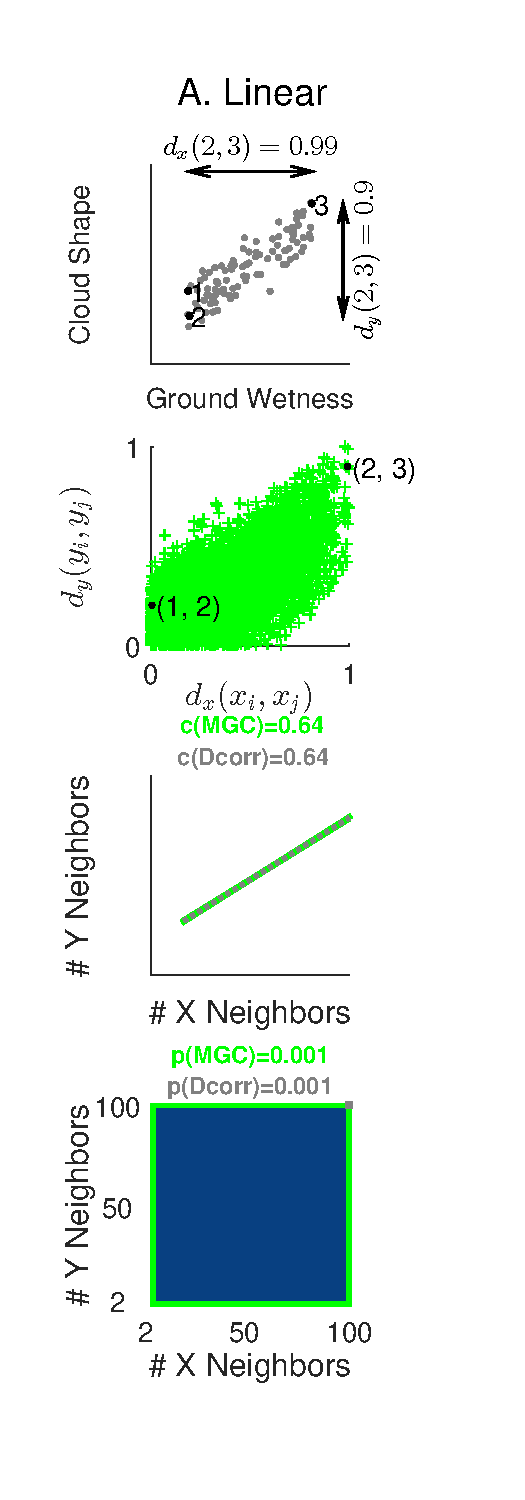
\includegraphics[width=1.0\textwidth]{../Figures/Fig1}
\caption{
Power of different methods on 20 different one-dimensional simulation settings, estimated on the basis of  10000 Monte-Carlo replicates.
Each panel shows empirical testing power on the absicca, and sample size on the ordinate.
LGC empirically achieves as high or higher power than the previous state of the art approaches for nearly all sample sizes on nearly all problems.}
\label{fig:1D}
\end{figure}


\subsection{High Dimensional Simulation Experiments}
\label{numer1}


For the increasing dimension scenario, LGC significantly surpasses all other methods: for dependencies that are close to linear, the powers of both dcorr and LGC deteriorate much slower than others; and for the remaining nonlinear dependencies, LGC is much better than all other methods including the mcorr, due to its capability to better handle non-linearity and high-dimensionality at the same time. Note that a quarter of the distributions (e.g. sine period, square, diamond) cannot be detected by any method at dimension higher than $1$, since all testing powers quickly degrade to around $\alpha$.

To intuitively summarize the simulation performance of each method in all settings, we apply the performance profiles introduced by \cite{DolanMore2002} to the testing powers, which is an evaluation tool to compare different algorithms throughout all given settings. Suppose there are $S$ methods and $T$ different settings, and we denote the respective powers as $\beta_{s}^{t}$ for $s=1,\ldots,S$ and $t=1,\ldots,T$. Then the relative performance for each method is defined as follows:
\begin{align*}
performance_{s}(x) &= \frac{1}{T} \sum_{t=1}^{T} I((\beta_{*}^{t}-\beta_{s}^{t}) \leq x)
\end{align*}
where $x \in [0,1]$ and $\beta_{*}^{t} =\max_{s} \beta_{s}^{t}$ denotes the best testing power in the $t$th setting. Namely $x$ stands for the difference with respect to the best power, and the performance profile of each method equals the proportion of simulations that the method is worse than the best method by no more than $x$. For example, at $x=0.1$, LGC has a relative performance of $0.75$ if and only if there are $15$ out of $20$ simulations that LGC is worse than the best method by no more than $0.1$ in testing power; the relative performance at $x=0$ stands for the proportion of simulations that the method has the best power; and the performance profile curve always increases to $1$ at $x=1$. The best method should have a similar or higher curve than others; and we also show the area under curve for each profile profile in the legend, which is a numerical way of viewing the advantage of each method.

In Figure~\ref{fig:pp} we show the performance profiles at fixed dimension and sample size that are determined by a power threshold, for both the dimension $1$ and increasing dimension scenarios. For the dimension $1$ scenario, the dimension is always fixed at $1$, so the sample size is determined by the first sample size that any method has a power of $0.8$ (otherwise pick the largest sample size); and for the increasing dimension scenario, the sample size is already fixed at $100$, so we determine the dimension choice by the first dimension that any method has a power that is lower than $0.5$ (otherwise pick the smallest dimension). The advantage of LGC does not change much with respect to the threshold choice, which can be seen from the AUC plot of performance profiles against the power threshold.


\begin{figure}[htbp]
\subfloat[]{
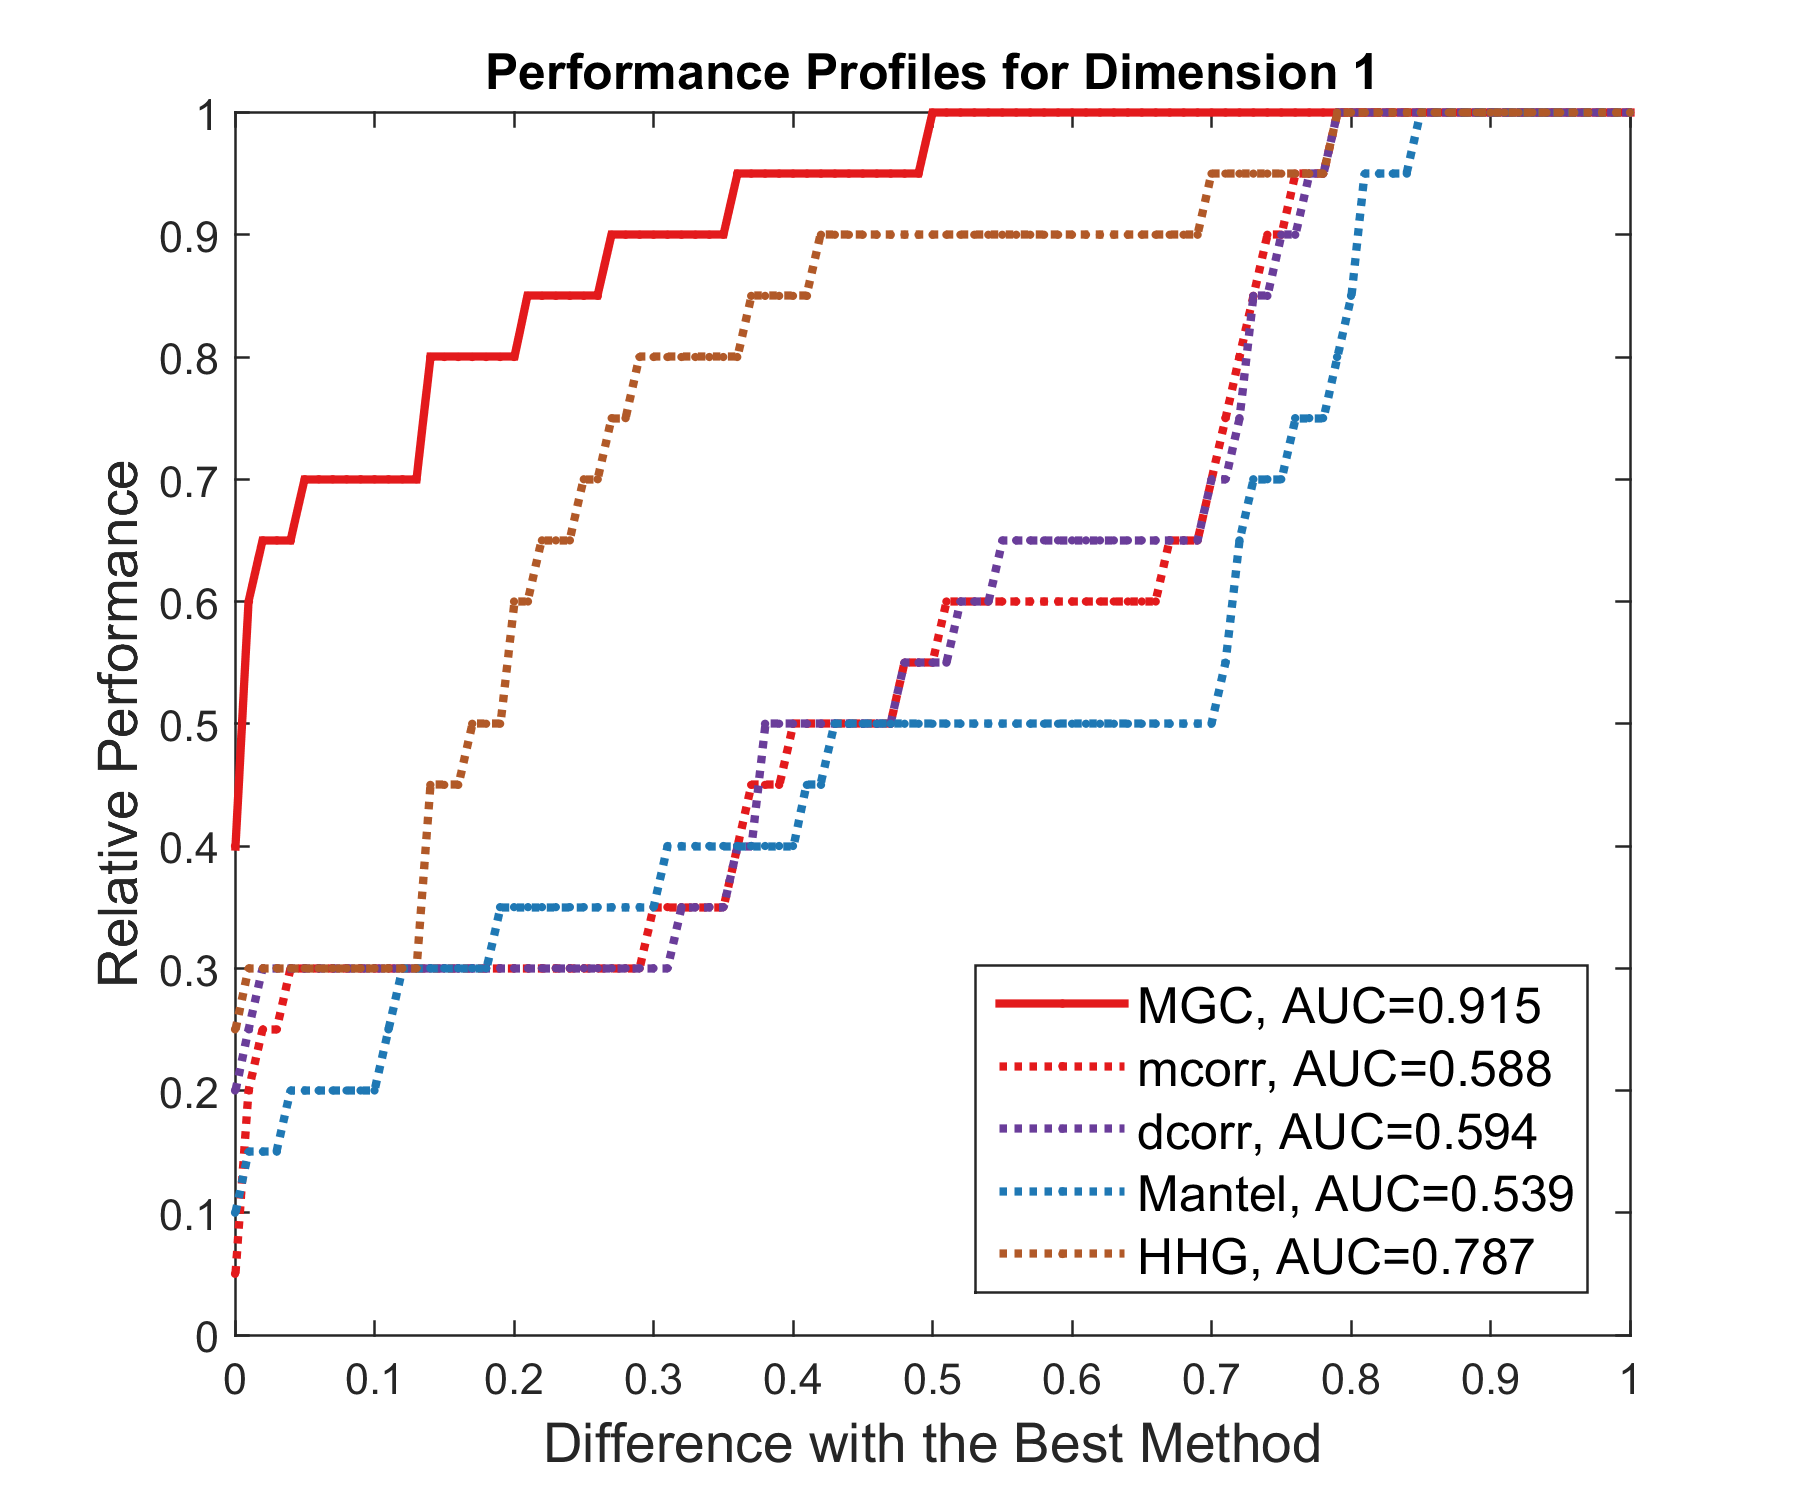
\includegraphics[width=0.5\textwidth]{../Figures/Fig3}
}
\hfil
\subfloat[]{
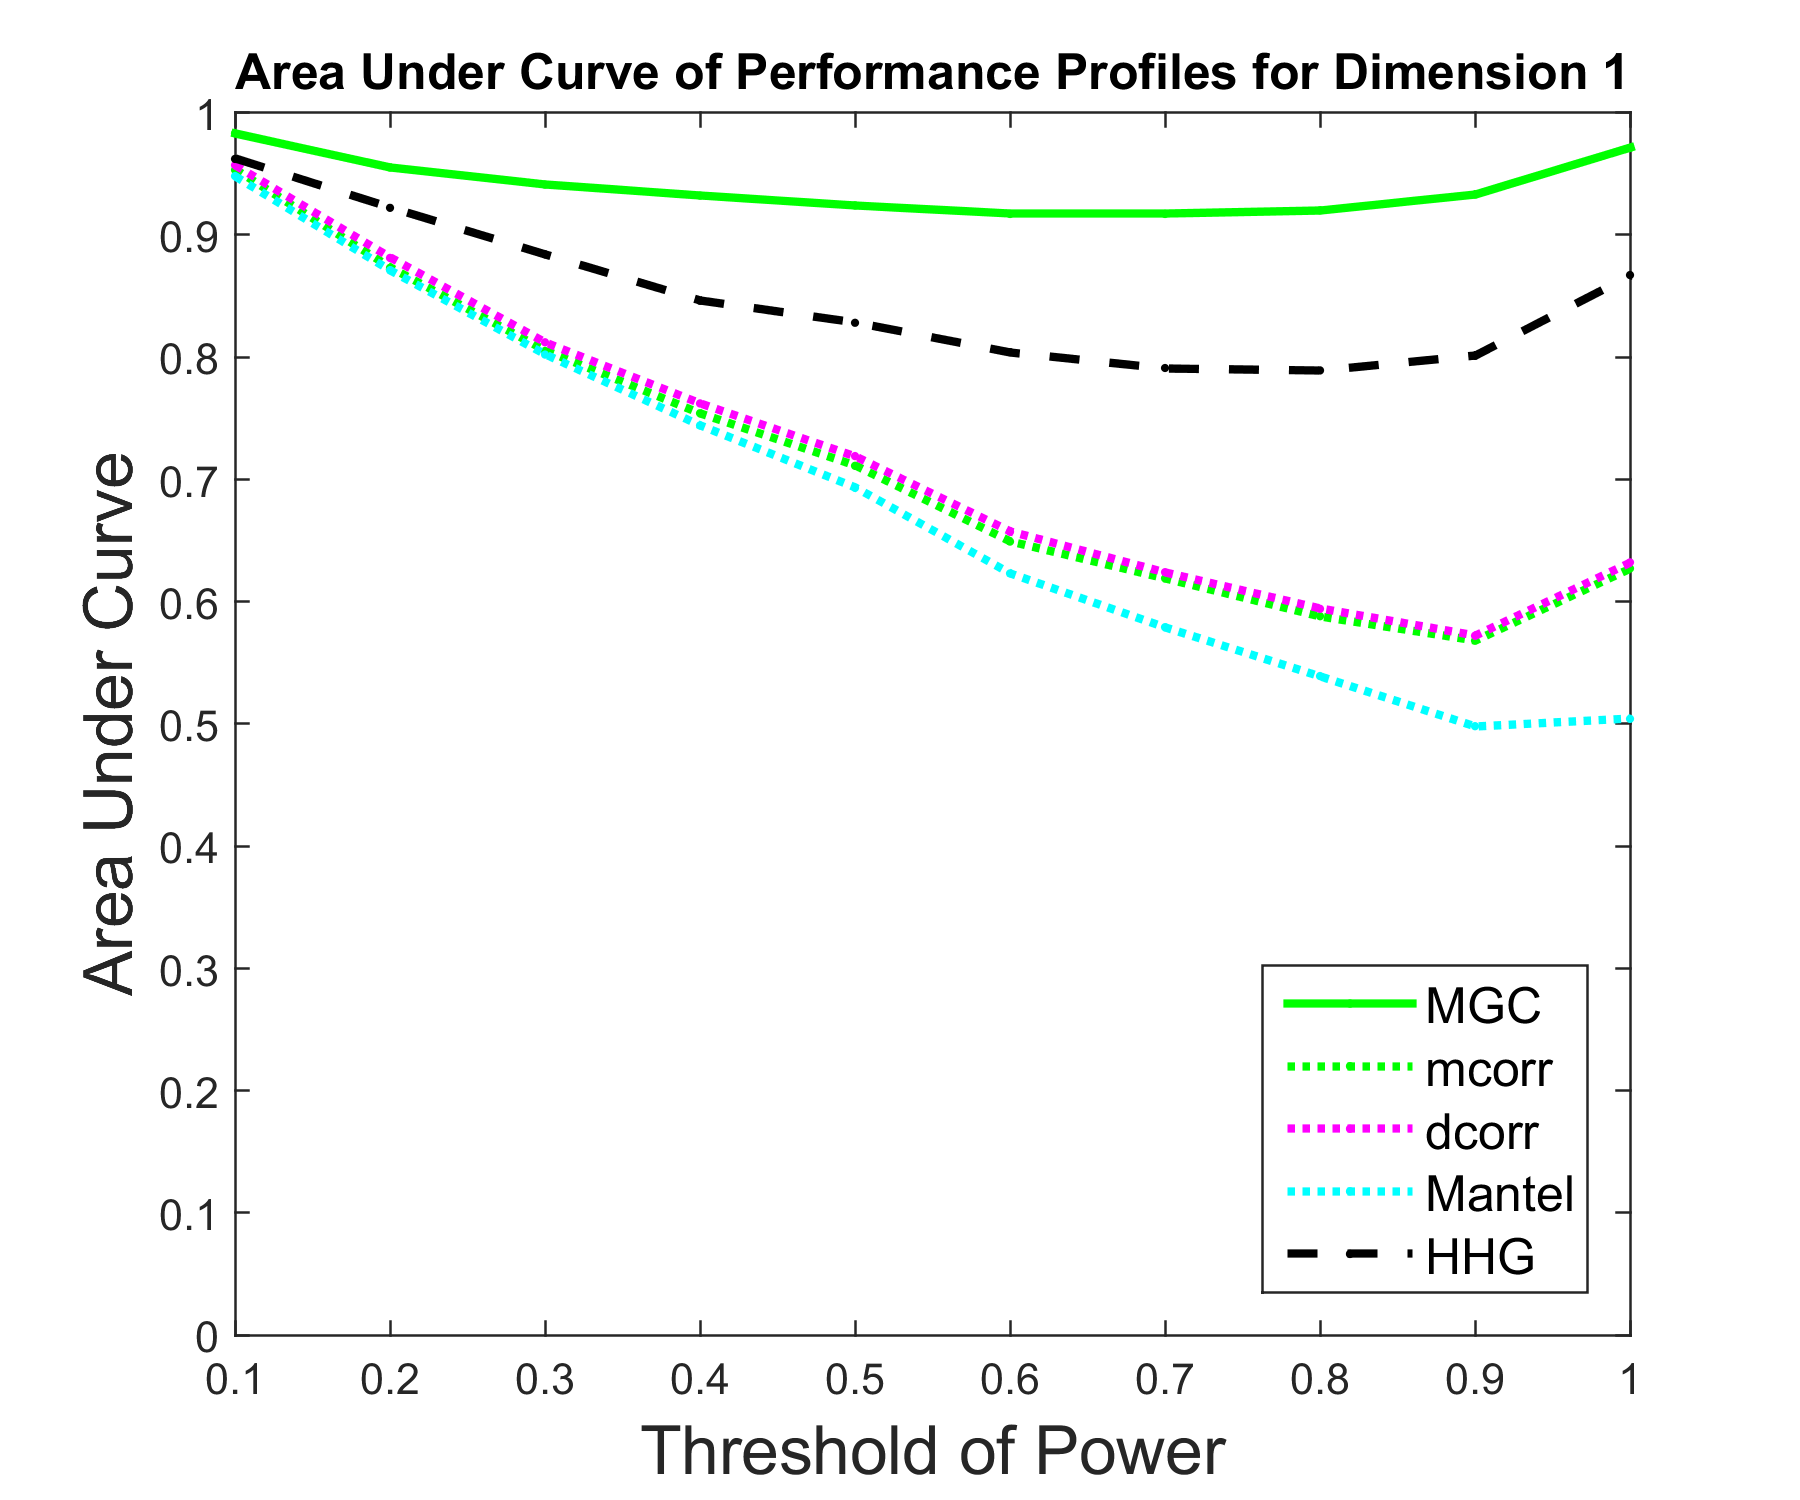
\includegraphics[width=0.5\textwidth]{../Figures/Fig4}
}
\hfil
\subfloat[]{
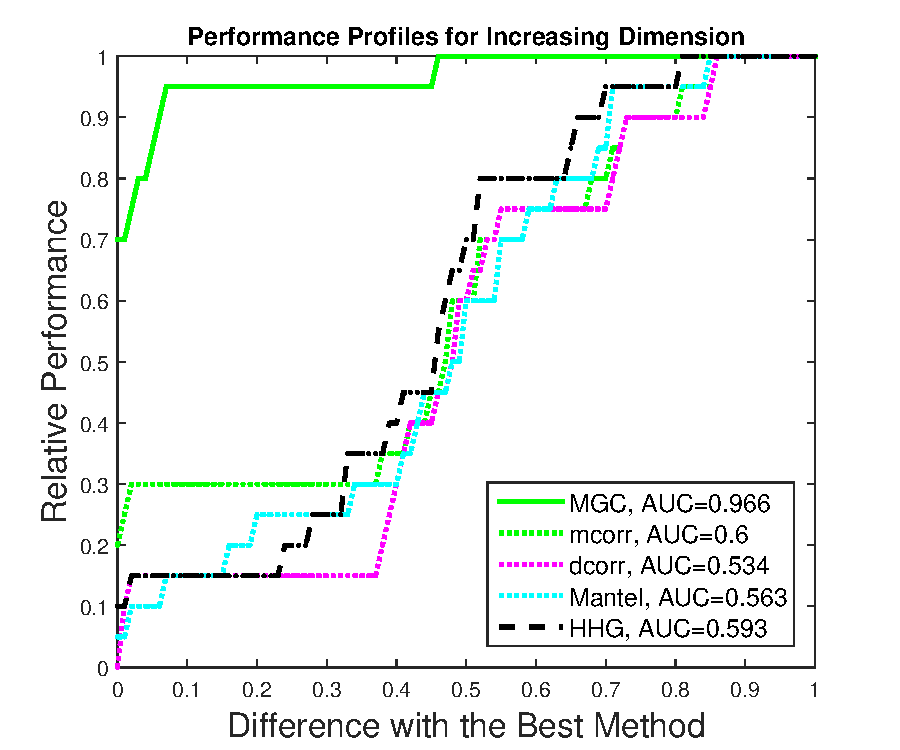
\includegraphics[width=0.5\textwidth]{../Figures/Fig7}
}
\hfil
\subfloat[]{
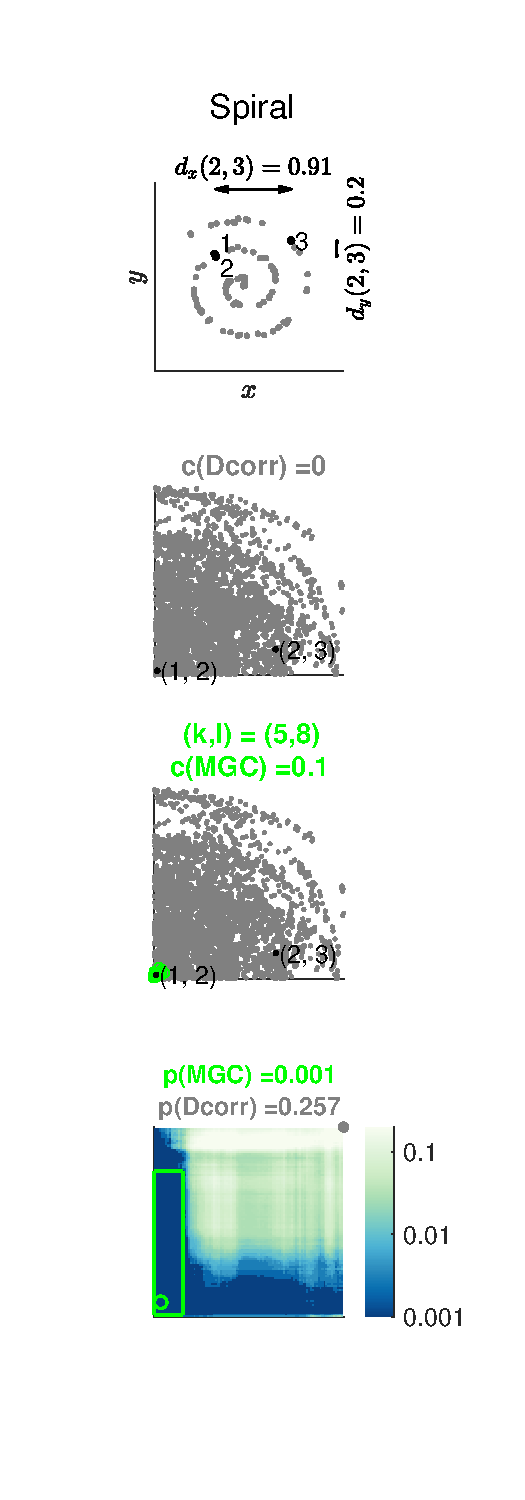
\includegraphics[width=0.5\textwidth]{../Figures/Fig8}
}
\caption{Quantitative comparisons of the power of the various algorithms across all simulations into a single number.  
(a) Performance profile plots comparing the different algorithms on all 1-dimensional problems at a fixed sample size where any testing power exceeds the power threshold 0.8. The legend provides the Area-Under-the-Curve (AUC) for each method; larger is better.
(b) AUC for each method sweeping over all different power thresholds.
(c) Same as (a) but for the high-dimensional simulations, YYY at a fixed dimension where any testing power drops below the power threshold 0.5 YYY XXX the previous clause is not clear to me XXX.
(d) Same as (b) but for the high-dimensional simulations.
It is clear that our method outperforms the previous state of the art, regardless of function, sample size, and dimensionality.}
\label{fig:pp}
\end{figure}

We can clearly see from Figure~\ref{fig:pp} that LGC is indeed the most reliable method in finite-sample testing, in accordance with the individual power plots in Figure~\ref{fig:1D} and Figure~\ref{fig:nD}. For the dimension $1$ scenario the performance profiles of LGC is clearly better than others, and for the increasing dimension scenario the advantage is even larger. Note that HHG is slightly better than dcorr in the performance profiles, because there are more nonlinear distributions than linear in the $20$ dependencies, and HHG has a larger advantage for nonlinear dependency than its disadvantage in linear dependency when compared to dcorr; and the Mantel test has the lowest performance profile in both scenarios. 




\begin{figure}[htbp]
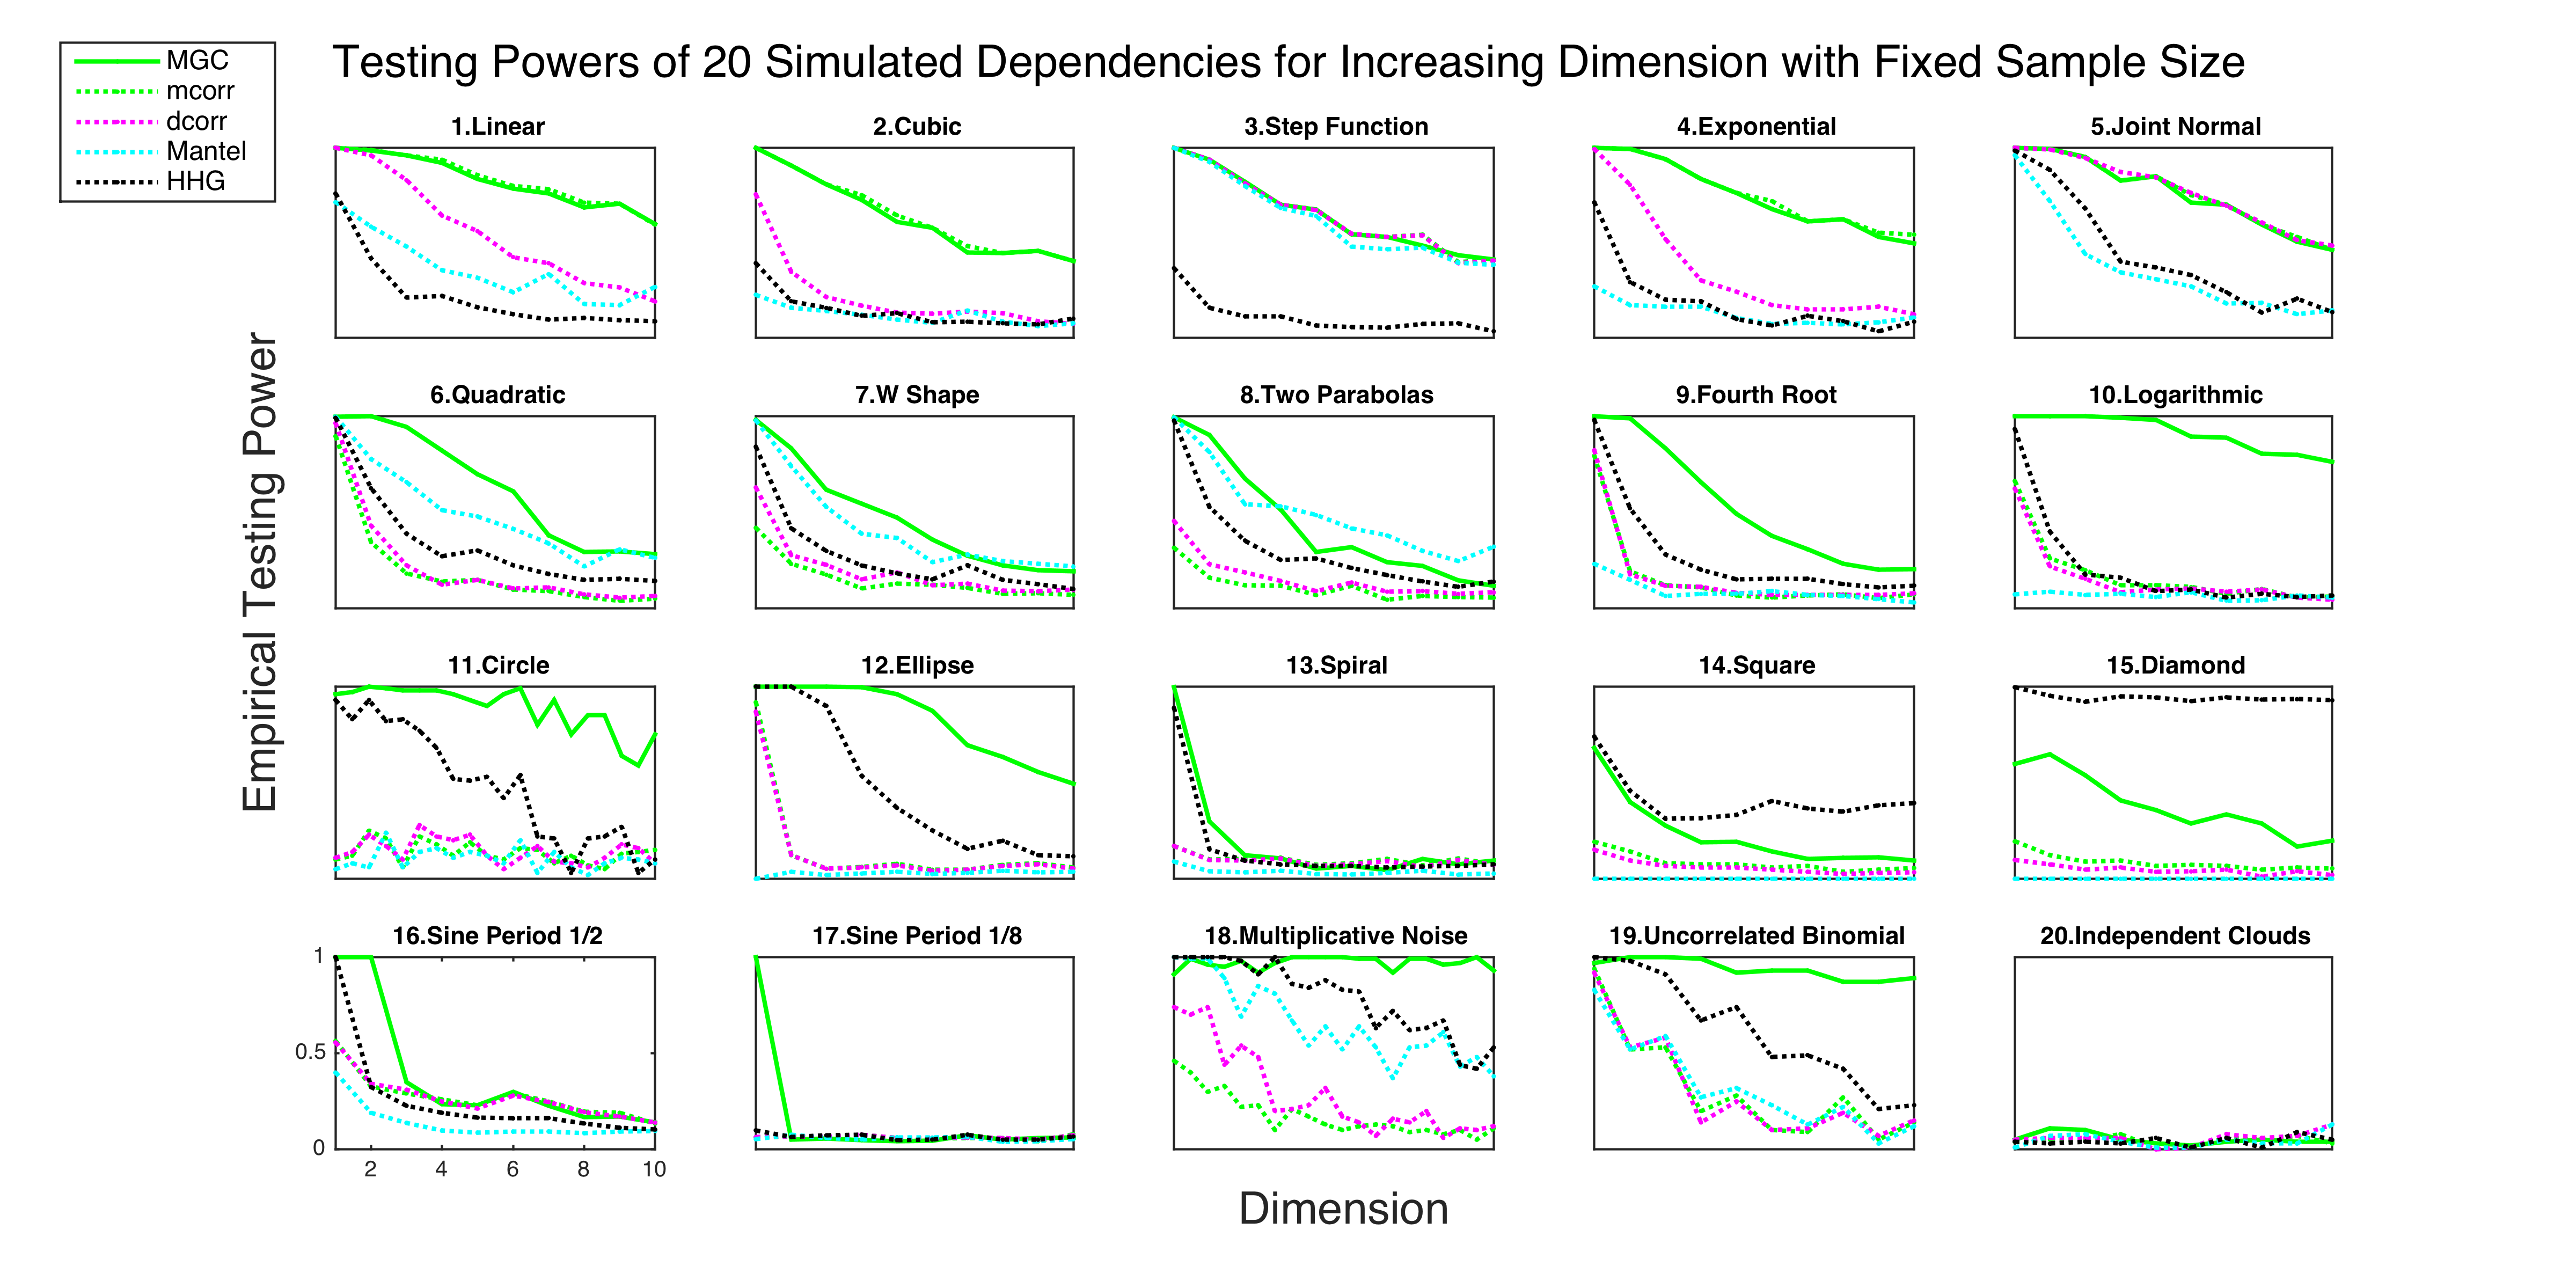
\includegraphics[width=1.0\textwidth]{../Figures/Fig5}
\caption{Power of different methods on 20 different simulation settings, for dimensionality ranging from 1 to 1000.  Details as in Figure~\ref{fig:1D}.
Again, our method empirically achieves as high or higher power than the previous state of the art approaches for nearly all sample sizes on nearly all problems and dimensions.
}
\label{fig:nD}
\end{figure}



\subsection{Discovery of Dependency Across Scales}

\begin{figure}[htbp]
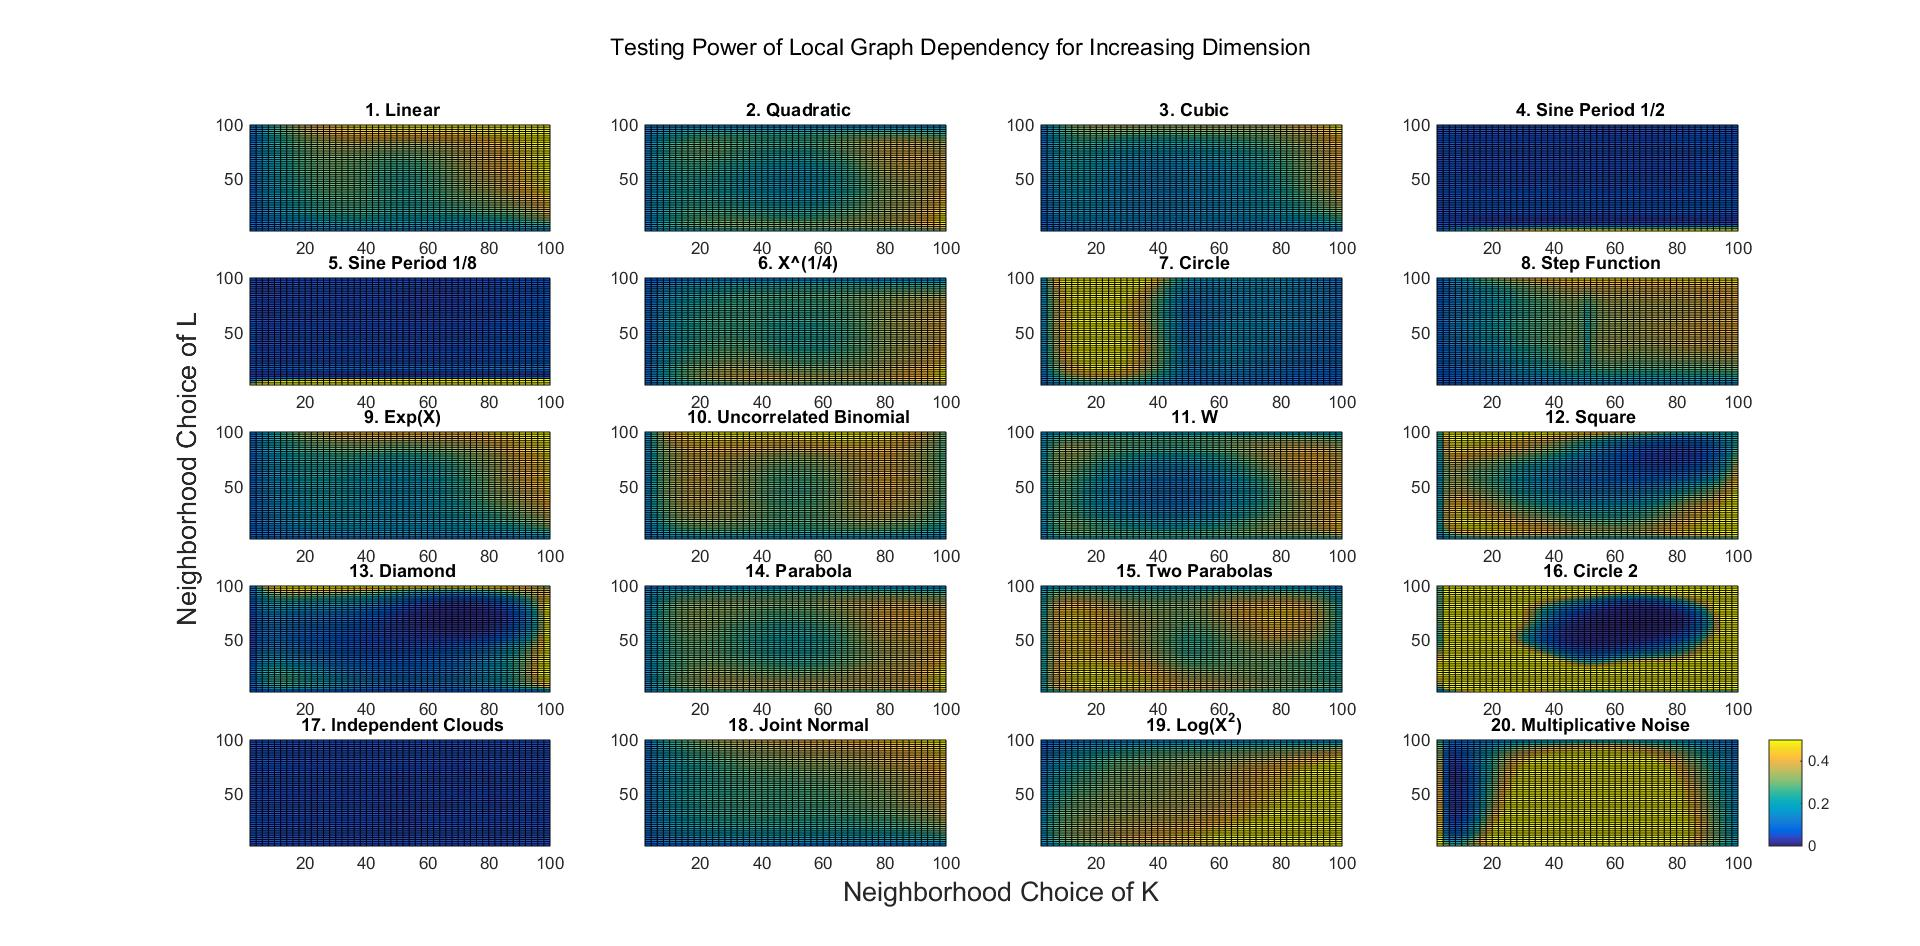
\includegraphics[width=1.0\textwidth]{../Figures/Fig6s}
\caption{Testing Power Heatmap of Local Graph Correlation for Increasing Dimension.
% Understanding how dependence varies with the local scale of the dependence.  
For each of the 20 panels, the abscissa denotes the number of neighbors for $X$, and the ordinate denotes the number of neighbors for $Y$.  Each different simulation yields a different surface, highlighting the importance of understanding local scale in terms of understanding the data. In almost all simulations, LDC outperforms the global special case.}
\label{figSim2}
\end{figure}
% \end{comment}







\subsection{Real Data}
\label{numer2}
Here we apply LGC to test independence between brain features and personal characteristics from two different experiments, for which the data sets are relatively small in sample size due to the expensive data collection process. 

The first experiment is to detect the relationship between the brain connectome and personality from \cite{AdelsteinEtAl2011}. The sample size is $n=42$, and each person has a $5$ dimensional personality data based on questionnaires and the five-factor personality model. Then the brain activity of each person is measured by fMRI for $197$ brain regions and $194$ time steps. Thus the brain connectome feature is high-dimensional while the personality data is low-dimensional. There seems to exist certain correlation between the brain activity and personality as experimentally shown in \cite{AdelsteinEtAl2011}, but whether the dependency can be detected from the raw data is the question here.

To apply our method, two distance measures are required for the two different data sources: for the personality data, the distance matrix $A$ is formed by the Euclidean distance directly; for the connectome data, we run a spectrum analysis for each region, bandpass and normalize it, then calculate the Kullback-Leibler divergence among regions and use the normalized Hellinger distance as the distance matrix $B$. Once the distance matrices $A$ and $B$ are obtained, we apply the permutation test in Section~\ref{main3} for $r=10000$ random permutations, and derive the p-values of LGC, dcorr, mcorr, and Mantel. 

The p-value by LGC is $0.0384$, for which the estimated neighborhood choice is $k=12, l=6$ based on $10000$ MC replicates. No other method yields significant (less than $0.05$) p-value, although HHG is quite close: dcorr has a p-value of 0.5863, mcorr has a p-value of 0.3217, HHG has a p-value of $0.0619$, and the Mantel test has a p-value of $0.9888$. We also show the p-value of LGC with respect to all possible neighborhood choice by heat map in the first plot of Figure~\ref{figReal}, and we can clearly see a local structure in the data that yield significant p-values for adjacent neighborhoods.

Note that if we use LGC based on dcorr rather than mcorr, the p-value becomes $0.4348$ achieved at $k=42, l=33$, which is no longer significant: this implies a high-dimensional structure in the dependency, which is indeed the case for the connectome data. Also note that the distance transformation (especially for the connectome data) may not be the most appropriate for detecting dependency, so it is possible that HHG and mcorr may yield better p-values for a different transformation.  XXX what do you mean distance ``transformation''?  seems like you mean ``distance''? or ``metric''? XXX


\begin{figure}[htbp]
\centering
\subfloat[]{
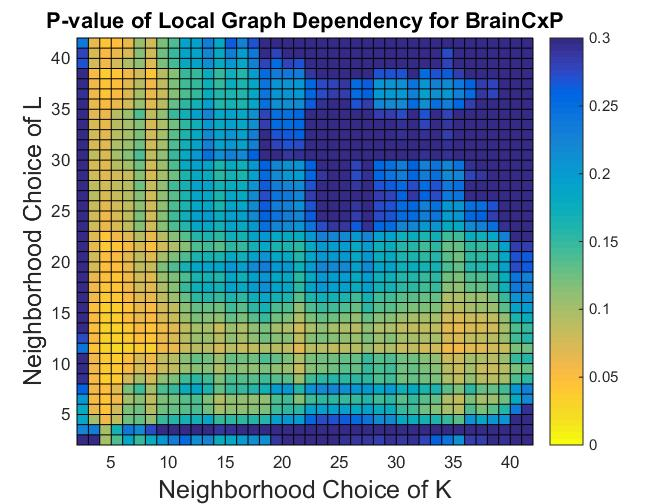
\includegraphics[width=0.48\textwidth]{../Figures/FigReal1Surface}
}
\hfil
\centering
\subfloat[]{
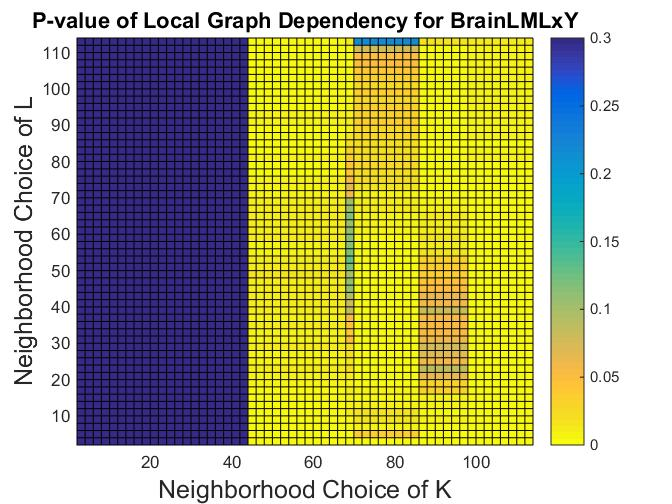
\includegraphics[width=0.48\textwidth]{../Figures/FigReal2Surface}
}
\hfil
\centering
\subfloat[]{
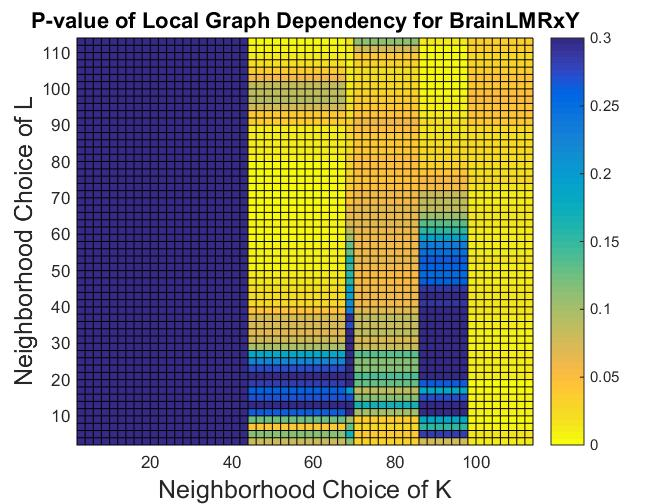
\includegraphics[width=0.48\textwidth]{../Figures/FigReal3Surface}
}
\caption{P-Value Heatmap of Local Graph Correlation with respect to Different Neighborhood Choice.  In the real data, for the personality vs. graph dependency, global structure is inadequate to reveal any dependence between the two modalities.  For the shape vs. status,  global distances are sufficient.  XXX we still need the example where we fail to detect dependence when it does not exist.  you have everything you need for that? XXX}
\label{figReal}
\end{figure}

Next we carry out the same testing procedure on another experiment regarding brain hippocampus shape and major depressive disorder. There are $n=114$ subjects, and the brain images of each person are obtained by  high resolution MRI scans on the hippocampus; and we also have available a categorical vector containing the disease information, including clinically depressed subject, high-risk subject, and non-affected subject. There has been evidences that relate major depressive disorder to the hippocampus shape in \cite{ParkEtAl2011} and \cite{PosenerEtAl2003}, and we would like to test the significance of such relationship in the data. 

The brain data is transformed into two dissimilarity matrices $LML$ and $LMR$, representing the left and right hippocampus data based on landmark matching (see \cite{ParkEtAl2011} for more details on data processing); and the label vector is transformed into its Euclidean distance matrix $D$, where $D(i,j)=0$ if and only if the $i$th subject has a different label from the $j$th subject. We consider two permutation tests: testing dependency between $LML$ and $D$, and testing dependency between $LMR$ and $D$.

For testing between the left brain and the disease, the p-value of LGC is $0.0010$ after $10$,$000$ random permutations, and the estimated neighborhood choice is $k=105,l=91$ based on $10$,$000$ MC replicates; dcorr has a p-value of $0.0448$, mcorr has a p-value of $0.0396$, HHG has a p-value of $0.0391$, and the Mantel test has a p-value of $0.0471$, so all benchmarks have larger p-values than LGC but are still significant at $0.05$. Note that the heat map of LGC with respect to different neighborhood choices is available in the second plot of Figure~\ref{figReal}; and if we use LGC based on dcorr instead, the p-value of LGC is still $0.0010$ at $k=106,l=92$ with a very similar heat map.

For testing between the right brain and the disease, the p-value of LGC is $0.0018$ with the estimated neighborhood choice being $k=106,l=91$; dcorr has a p-value of $0.0750$, mcorr has a p-value of $0.0758$, HHG has a p-value of $0.0859$, and the Mantel test has a p-value of $0.0765$, so all benchmarks are not significant at $0.05$. Note that the heat map of LGC with respect to different neighborhood choices is available in the third plot of Figure~\ref{figReal}; and if we use LGC based on dcorr instead, the p-value of LGC becomes $0.0016$ at $k=105,l=92$.

XXX Insert a table showing the p-value for each of the methods across each of the settings. XXX

We can observe from the heat map of LGC that there is a clear threshold in the local structure most neighborhood choices after certain threshold yields significant p-values, and LGC with mcorr performs similarly as LGC with dcorr. They imply that the dependency between the brain data and the disease data is probably cross-region, close to linear and low-dimensional. Furthermore, the left brain seems to be more correlated with the disease than the right brain, as testing between $LML$ and $D$ yields smaller p-values than testing between $LMR$ and $D$.
YYY cross-region means: if we limit our observation within a small region in this data, there won't be any dependency; and there is a significant jump in p-value after certain neighborhood threshold YYY XXX i don't understand why you believe these results imply anything about cross-regional dependencies? because k,l are large? so we need to incorporate distances that are big? i think it might be a cool insight, i just don't understand it. XXX

Note that the p-value is always $0$ for any test statistic when testing independence between $LML$ and $LMR$, implying strong linear dependency between the left and right brain.

\section{Discussion}
\label{conclu}

\paragraph{Summary}

In short, we propose local graph correlation to test independence between data sets, which has been shown to be perform well for testing independence on data of small sample size, high-dimensionality, linearity or non-linearity. It not only enjoys theoretical guarantee such as being consistent in testing independence, but also exhibits superior numerical performances in a comprehensive simulation setting and real data experiments, comparing to other popular methods.


\paragraph{Next Steps}

one-sample, two-sample, group testing, anova, regressing out other covariates (local partial correlation), screening, metric spaces.

different test statistics: there are many possible ways to generate the null distribution, including permutation, but also t-test (as in the mdcorr paper and the asymptotic distribution derived from Gretton et al 2009), wilcoxon signed rank test, etc..


scaling up via FlashX?

\section*{Acknowledgment}
\addcontentsline{toc}{section}{Acknowledgment}
This work was partially supported by 
% 
National Security Science and Engineering Faculty Fellowship (NSSEFF), 
% 
Johns Hopkins University Human Language Technology Center of Excellence (JHU HLT COE), 
% 
Defense Advanced Research Projects Agency's (DARPA) SIMPLEX program through SPAWAR contract N66001-15-C-4041, 
% 
and the XDATA program of the Defense Advanced Research Projects Agency (DARPA) administered through Air Force Research Laboratory contract FA8750-12-2-0303.



\appendix

\section{Functions}

\begin{figure}[htbp]
\subfloat[]{
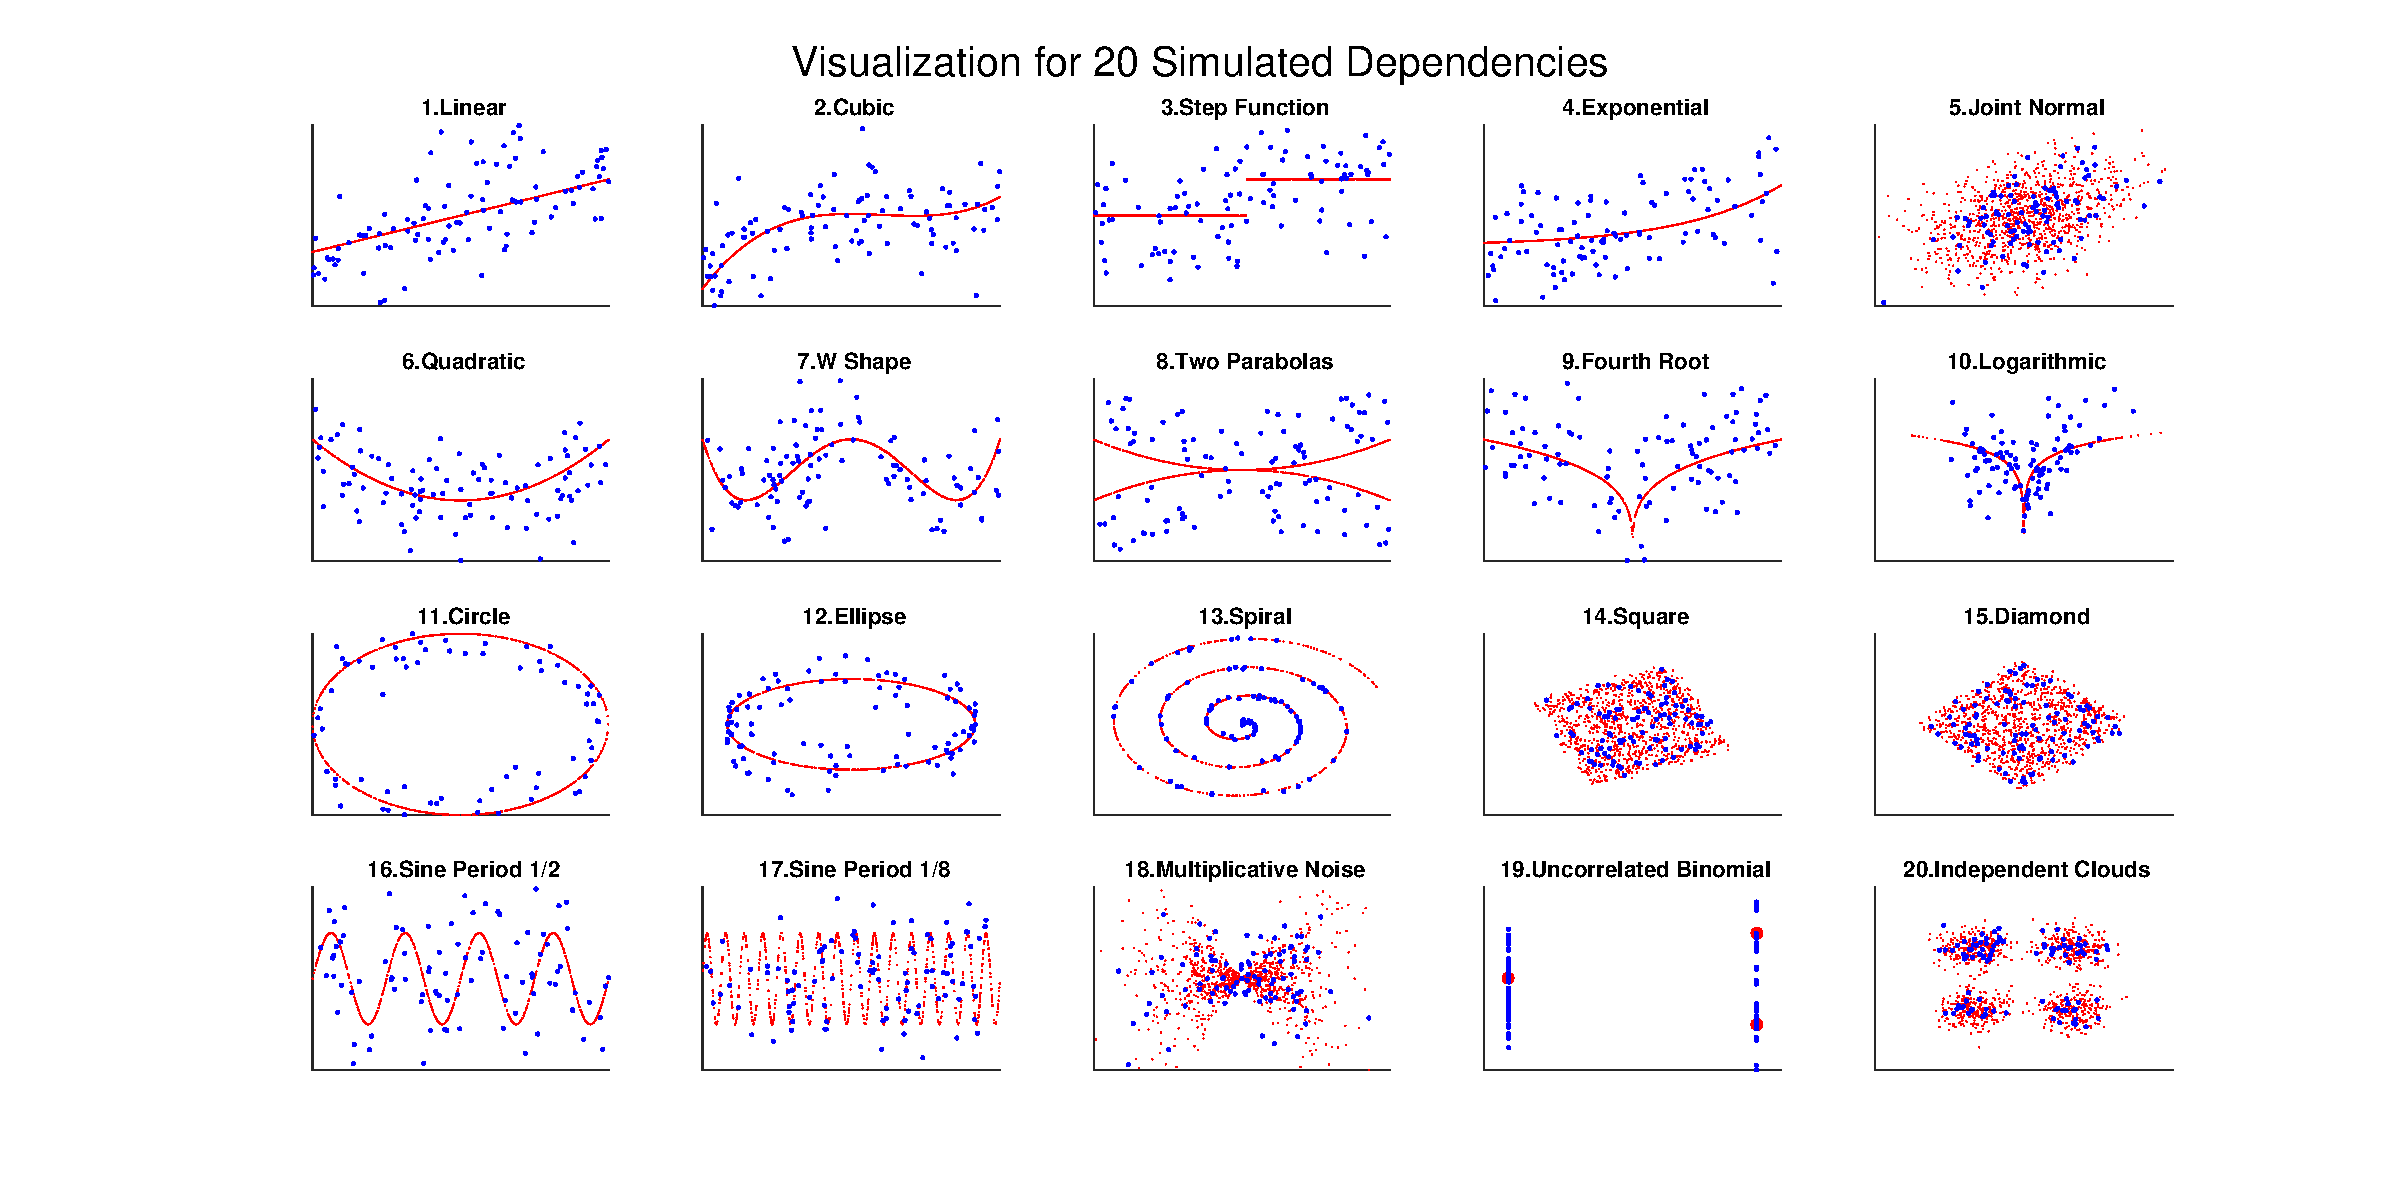
\includegraphics[width=1.0\textwidth]{../Figures/Fig0}
}
\caption{Visualization of 20 different at dimension $1$ and $n=1000$ with no noise}
\label{fig0}
\end{figure}


\section{Supplementary Figures}
\begin{figure}[htbp]
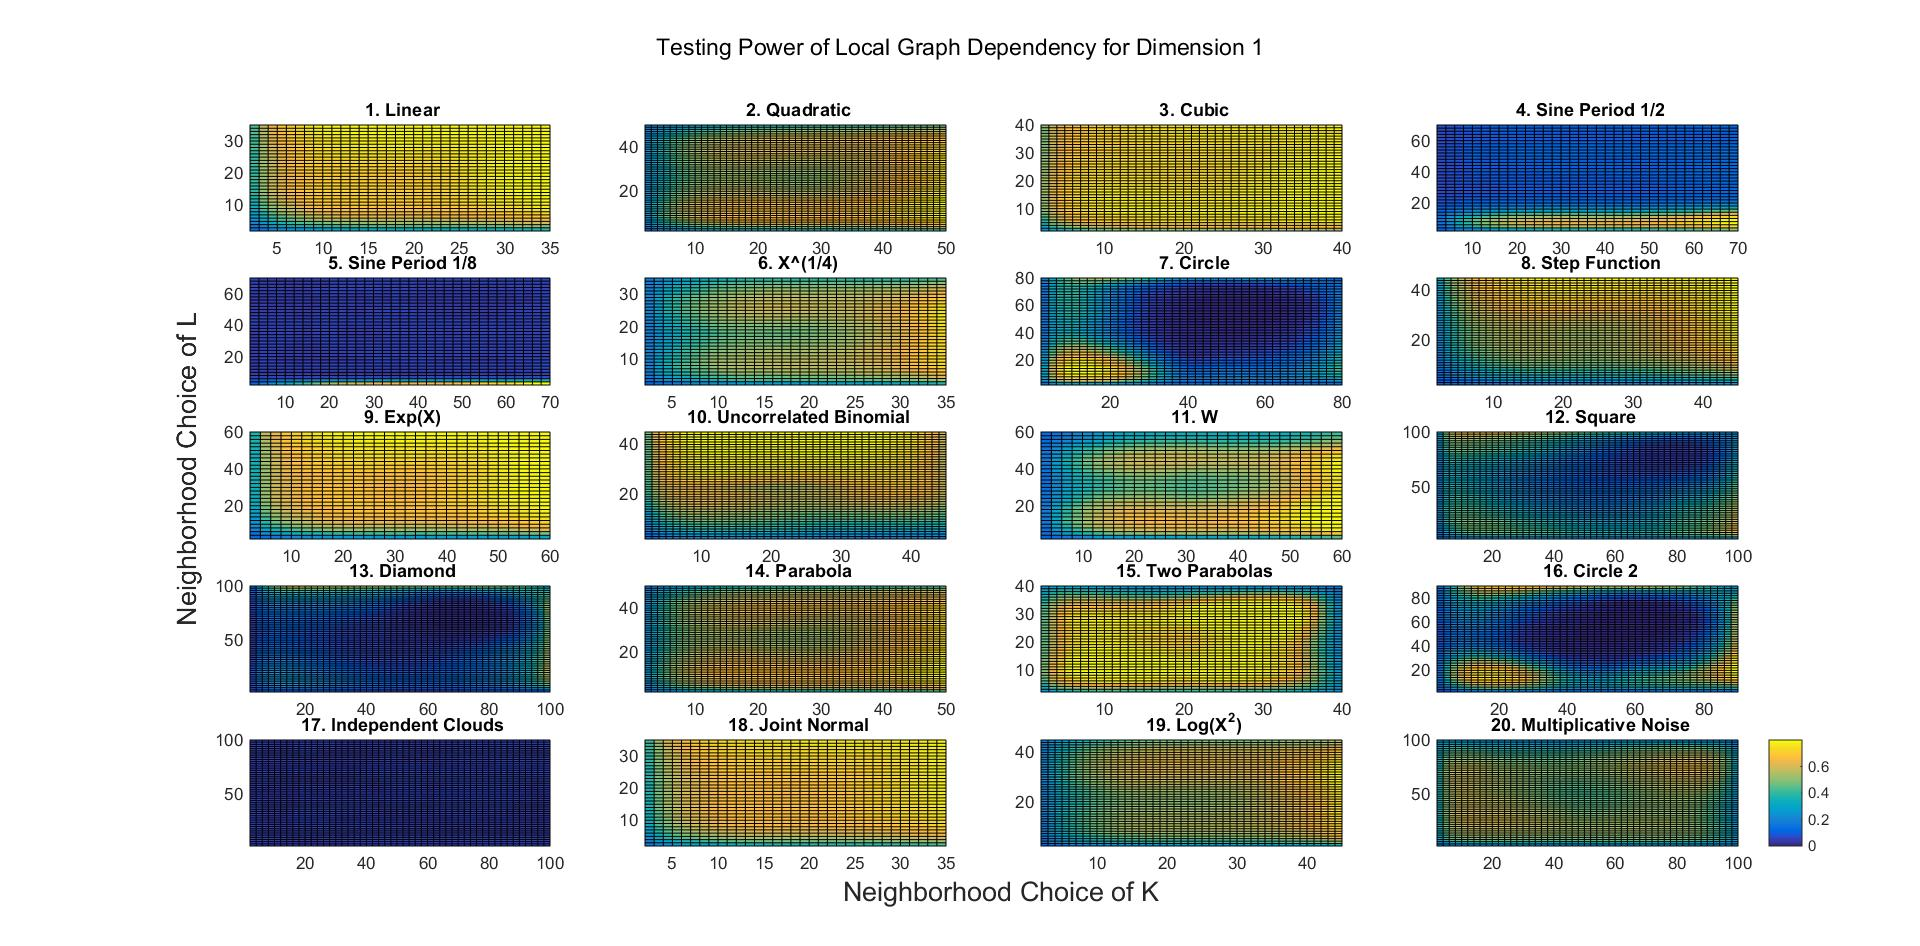
\includegraphics[width=1.0\textwidth]{../Figures/Fig2s}
\caption{Testing Power Heat-map of Local Graph Correlation for Dimension 1}
\label{figSim2}
\end{figure}


\section{Data Collection}


\section{Dependence Measures}
\label{main}

XXX I like the following notations:

$x_i \in \mc{X} \subset \Real^{d_x}$, $\mb{x} \sim F_x$, and $X=\{x_1,\ldots,x_n\}$ and similarly for $y$. then $A=(a_{ij})$. 

so, lower case for scalars, caps for vectors and matrices, bold for random variables, and script for spaces.  

i'd let the centered distances be denote $A^H$ and the modified ones $A^M$.
and the local ones $\mt{A}$.

i'm open to other consistent conventions, but you sometimes write $A_{ij}$ to mean the scalar (un-center and normalized distance), which i think is confusing.
XXX


Suppose we are given two data sets $\mathcal{X}=[X_{1},\cdots, X_{n}] \in \mathcal{R}^{m_{X} \times n}$ and $\mathcal{Y}=[Y_{1},\cdots, Y_{n}] \in \mathcal{R}^{m_{Y} \times n}$, where $n$ is the sample size, $m_{X}$ and $m_{Y}$ are the dimensions for each data set. Under the classical hypothesis testing framework, we assume that $X_{i}, i=1,\ldots,n$ are identically independently distributed (iid) acoording to $f_X$, similarly $Y_{i} \stackrel{iid}{\sim} f_Y$. Throughout the paper, we always assume that $X$ and $Y$ have finite second moments, which is a necessary assumption to guarantee the consistency of distance correlation.

For testing independence between $X$ and $Y$, the null and the alternative hypothesis are
\begin{align*}
& H_{0}: f_{XY}=f_{X}f_{Y},\\
& H_{A}: f_{XY} \neq f_{X}f_{Y},
\end{align*}
where $f_{XY}$ denotes the joint distribution of $(X,Y) \in \mathcal{R}^{m_{X}+m_{Y}}$, and $f_{X}$ and $f_{Y}$ are the marginal distributions. 


\subsection{Mantel Test}
\label{sec:hhg}



The other method we use as the benchmark in the numerical section is the Mantel test, which simply applies Pearson's product-moment correlation coefficient  to the distance matrices, see in \cite{Mantel1967}. Despite its lack of theoretical guarantee (for example, unlike distance correlation and HHG, it is not consistent against all alternatives), it has been a very popular method so far and commonly used in biology and ecology. In our numerical simulations we will observe that the Mantel test is not consistent for many nonlinear dependencies, and is sub-optimal in almost all types of dependency we consider.

XXX i don't know what ``applies pearson's to a distance matrix''.  i mean, \emph{i} know what you mean, but i don't think it is clear.  also, where the null distribution comes from is not clear.  XXX



\subsection{Global Distance Correlation}
\label{main1}


To test independence by distance correlation on sample data, we first calculate two Euclidean distance matrices $A, B \in \mathcal{R}^{n \times n}$ for $\mathcal{X}$ and $\mathcal{Y}$ respectively, i.e., $A_{ij}=\|X_{i}-X_{j}\|_{2}$. The sample distance covariance is defined as
\begin{equation}
\label{dCovEqu}
dCov_{n}(\mathcal{X},\mathcal{Y})=\frac{1}{n^2}\sum_{i,j=1}^{n}A^{H}_{ij}B^{H}_{ij},
\end{equation}
where $A^{H}=HAH$, $B^{H}=HBH$ with $H=I_{n}-\frac{J_{n}}{n}$. Then the sample distance variance is defined as
\begin{align*}
dVar_{n}(\mathcal{X}) &=\frac{1}{n^2}\sum_{i,j=1}^{n}A^{H}_{ij}A^{H}_{ij}\\
dVar_{n}(\mathcal{Y}) &=\frac{1}{n^2}\sum_{i,j=1}^{n}B^{H}_{ij}B^{H}_{ij}.
\end{align*}
The squared sample distance correlation is obtained by normalizing the distance covariance
\begin{equation}
\label{dCorrEqu}
dCorr_{n}(\mathcal{X},\mathcal{Y})=\frac{dCov_{n}(\mathcal{X},\mathcal{Y})}{\sqrt{dVar_{n}(\mathcal{X}) \cdot dVar_{n}(\mathcal{Y})}},
\end{equation}
where all of $dCov_{n}, dVar_{n}, dCorr_{n}$ are always non-negative. Note that the $dCov_{n}/dCorr_{n}$ above is actually the square of distance covariance/correlation in \cite{SzekelyRizzoBakirov2007}; but for simplicity we drop the square in the name throughout this paper.

It is shown in \cite{SzekelyRizzoBakirov2007} that as $n \rightarrow \infty$, $dCorr_{n}(\mathcal{X},\mathcal{Y}) \rightarrow dCorr(X,Y) \geq 0$, where $dCorr(X,Y)$ is the population distance correlation of $X$ and $Y$ defined by their characteristic functions. The population distance correlation is $0$ if and only if $X$ and $Y$ are independent, so that the sample distance correlation is a consistent test for independence, i.e., the testing power converges to $1$ as $n$ increases, at any fixed type $1$ error level. Note that in this paper distance correlation always means the sample statistic rather than the population statistic, unless otherwise mentioned.

\subsection{Global Modified Distance Correlation}
\label{sec:gmd}


However, in case of high-dimensional data where the dimension $m_{X}$ or $m_{Y}$ increases with the sample size $n$, the original distance correlation $dCorr_{n}$ is no longer appropriate. For example, even for independent Gaussian distribution, $dCorr_{n} \rightarrow 1$ as $m_{X}, m_{Y} \rightarrow \infty$, such that it is no longer a consistent test in high dimension. This problem is solved by the modified distance correlation proposed in \cite{SzekelyRizzo2013a}:
\begin{equation}
\label{mdCovEqu}
mdCov_{n}(\mathcal{X},\mathcal{Y})=\frac{1}{n(n-3)}(\sum_{i \neq j}^{n}A^{H*}_{ij}B^{H*}_{ij}-\frac{2}{n-2}\sum_{i=1}^{n}A^{H*}_{ii}B^{H*}_{ii}),
\end{equation}
where $A^{H*}_{ij}$ adjusts the entries of $A^{H}$ by
\[A^{H*}_{ij} = \left\{
  \begin{array}{lr}
    \frac{n}{n-1}(A^{H}_{ij}-\frac{A_{ij}}{n}), & \mbox{ if } i \neq j \\
    \frac{1}{n-1}(\sum_{i}A_{ij}-\frac{\sum_{i,j}A_{ij}}{n}), &\mbox{ if } i = j
  \end{array}
\right.
\] 

XXX why is there a $\frac{n}{n-1}$ both inside the sum, and another right outside the sum? let's put it inside or outside, but not both? XXX 
YYY explanation: there is only one $\frac{n}{n-1}$ out side the sum? YYY
and similarly for $B^{H*}_{ij}$. Then $mdVar_{n}(\mathcal{X})$ can be defined by replacing all $B^{H*}_{ij}$ in Equation~\eqref{mdCovEqu} by $A^{H*}_{ij}$, similarly define $mdVar_{n}(\mathcal{Y})$. 

If $mdVar_{n}(\mathcal{X}) \cdot mdVar_{n}(\mathcal{Y}) \leq 0$, the modified distance correlation is set to $0$ (negativity can only occur when $n\leq 2$, equality can only happen in very special cases); otherwise it is defined as
\begin{equation}
\label{mdCorrEqu}
mdCorr_{n}(\mathcal{X},\mathcal{Y})=\frac{mdCov_{n}(\mathcal{X},\mathcal{Y})}{\sqrt{mdVar_{n}(\mathcal{X}) \cdot mdVar_{n}(\mathcal{Y})}}.
\end{equation}
It is shown in \cite{SzekelyRizzo2013a} that $mdCorr_{n}(\mathcal{X},\mathcal{Y})$ is an unbiased estimator of the population distance correlation $dCorr(X,Y)$ for all $m_{X}, m_{Y}, n$; and $mdCorr_{n}$ is approximately normal even if $m_{X},m_{Y} \rightarrow \infty$. Thus it is also a consistent test of independence, which works better than the original distance correlation in high-dimension.


To summarize this subsection, both the distance correlation and modified distance correlation are great for testing independence of Euclidean data due to their theoretical consistency, with the modified test statistic being more robust against high-dimensional dependency. Indeed it is a flourishing concept by a series of papers \cite{BakirovRizzoSzekely2006, SzekelyRizzoBakirov2007, SzekelyRizzo2009, BickelXu2009, Kosorok2009, Remillard2009, LiZhongZhu2012, SzekelyRizzo2013a, SzekelyRizzo2013b, SzekelyRizzo2014}; and the test statistic is not limited to the Euclidean metric as shown in \cite{Lyons2013}. 

XXX sorry i was unclear.  i don't know what ``robust against high-dimensional dependency'' means. when i say ``robust'', i always mean with respect to a model, for which the dimensionality is an intrinsic property.  eg, robust against contamination, eg, points sampled from a different model (but in the same space). i'd say something like, ``exists impressive finite sample performance even under high-dimensional settings'', or ``combats the curse of dimensionality via...''XXX

However, the required sample size for achieving a good testing power very much depends on the type of dependency underlying the given data, e.g. for perfect linear relationship, sample distance correlation usually requires less than $10$ points for a permutation test to declare significance; but for some nonlinear relationships like circle, sample distance correlation yields no significance even at $n=100$. Because real data rarely exhibits perfect linear relationship, and in practice large amount of data may not always be available, a better finite-sample method is of tremendous value: it not only yields a better testing power for the same sample size, but may also requires much less sample data for the permutation test to declare significance, which in turn saves the running time and data collection process. 


\subsection{Heller, Heller \& Gorfine (HHG)}
\label{sec:hhg}


There exists another distance-based method that is consistent and works particularly well for nonlinear dependencies, which is called the HHG statistics in \cite{HellerGorfine2013}. It applies Pearson's chi-square test to ranks of distances within each column rather than directly summing up the products of distances, and is shown to be better than distance correlation and other methods for finite-sample testing of many common nonlinear relationships in \cite{GorfineHellerHeller2012} and \cite{HellerGorfine2013}. However, in our numerical simulations HHG seems to fall a bit short when testing against high-dimensional or close to linear dependency, but is otherwise a strong competitor of the global distance correlation. 


\section{Local Distance Correlation}
\label{main2}

Since there has not been a method that perform well against all possible alternatives in finite-sample testing, it motivates us to propose a local distance correlation that is concurrently robust against small sample size, high-dimensionality, linearity or non-linearity in the following subsection.


In this subsection we define the local distance correlation, which is based on k-nearest-neighbor and applicable to both the original distance correlation and the modified distance correlation. From now on, we distinguish the local test statistic as either the local original distance correlation or the local modified distance correlation when they have different behaviors in the context, otherwise we call both as local/global distance correlation since they often share the same properties.

Under the same setting and notation as the global distance correlation in Section~\ref{main1}, we further sort the distance matrix $A$ within column and denote the ranks as $r(A_{ij})$: for each $i=1, \ldots, n$, we always set $r(A_{ii})=0$; then set $r(A_{ij})=k$ if and only if $A_{ij}$ is the $k$th smallest distance in $\{A_{ij}, i=1,\ldots,n\ \& \ i \neq j\}$; for ties, we take the minimum rank among them (this is of importance for local modified distance correlation, see explanation below). Similarly sort the distance matrix $B$ within column and denote the ranks by $r(B_{ij})$.

Then for each $k,l=1,\ldots,n$, we can calculate a ``local'' version of distance covariance as
\begin{equation}
\label{localdCovEqu}
dCov_{kl}(\mathcal{X},\mathcal{Y})=\frac{1}{n^2}\sum_{i,j=1}^{n}A^{H}_{ij}B^{H}_{ij}I(r(A_{ij})<k)I(r(B_{ij})<l),
\end{equation}
and calculate a local version of distance variance as
\begin{align*}
dVar_{k}(\mathcal{X}) &=\frac{1}{n^2}\sum_{i,j=1}^{n}A^{H}_{ij}A^{H}_{ij}I(r(A_{ij})<k)\\
dVar_{l}(\mathcal{Y}) &=\frac{1}{n^2}\sum_{i,j=1}^{n}B^{H}_{ij}B^{H}_{ij}I(r(B_{ij})<l),
\end{align*}
where $I(\cdot)$ is the indicator function. After normalizing, we have a family of distance correlation:
\begin{equation}
\label{localdCorrEqu}
dCorr_{kl}(\mathcal{X},\mathcal{Y})=\frac{dCov_{kl}(\mathcal{X},\mathcal{Y})}{\sqrt{dVar_{k}(\mathcal{X}) \cdot dVar_{l}(\mathcal{Y})}}.
\end{equation}
When $k=l$, we simplify the notations to $dCov_{k}$ and $dCorr_{k}$; and the family of local test statistics $\{dCorr_{kl}, k,l=2,\ldots,n\}$ includes the original distance correlation $dCorr_{n}$ as well. Note that in the family we exclude $dCorr_{1l}$ and $dCorr_{k1}$, because it holds that $dCorr_{1l}=dCorr_{k1}=dCorr_{11}$, which does not consider any neighbor, merely counts the diagonal terms in the distance matrices, and not meaningful for testing independence.

From now on, local distance correlation refers to the family of the test statistics $\{dCorr_{kl}, k,l=2,\ldots,n\}$ rather than each individual $dCorr_{kl}$; and the testing power of local distance correlation refers to the best testing power achieved in the family. Since $k,l$ are finite, the optimal testing power always exists; and it is clear that the optimal power and the corresponding best local test statistic are dependent on the joint distribution $f_{XY}$ and may not be unique.

In the same manner, we can apply the above to modified distance covariance:
\begin{equation}
\label{localmdCovEqu}
mdCov_{kl}(\mathcal{X},\mathcal{Y}) =\frac{1}{n(n-3)}(\sum_{i \neq j}^{n}A^{H*}_{ij}B^{H*}_{ij}I(0<r(A_{ij})<k)I(0<r(B_{ij})<l)-\frac{2}{n-2}\sum_{i=1}^{n}A^{H*}_{ii}B^{H*}_{ii}), 
\end{equation}
then $mdCorr_{kl}$ is obtained by normalizing each $mdCov_{kl}(\mathcal{X},\mathcal{Y})$ by the square root of $mdVar_{k}(\mathcal{X}) \cdot mdVar_{l}(\mathcal{Y})$; $0$ if the square root is either $0$ or not a real number. It follows that local modified distance correlation refers to the family $\{mdCorr_{kl}, k,l=2,\ldots,n\}$. Note that by using the minimal rank among ties, the summation of Equation~\eqref{localmdCovEqu} never includes repeated points: as the advantage of modified distance correlation mostly lies in its exclusion of the diagonal distance products, when ties occur in the data, there will be multiple zero distance terms other than the diagonal such that including those repeated points (i.e., points of column rank $0$) significantly inflate $mdCov_{kl}$ and negates the advantage of the modification; so this change is necessary for local modified distance correlation to function properly in practice, since our bootstrap procedure in the permutation test almost always produce ties in the re-sampled data.

Because $\{mdCorr_{kl}\}$ has the same asymptotic properties as $\{dCorr_{kl}\}$ other than its robustness against high-dimensionality, we will mostly use $\{dCorr_{kl}\}$ for explanation purposes in Section~\ref{main}. Indeed in the numerical section, local modified distance correlation has similar numerical performance as the local original distance correlation at dimension $1$, but much more superior at higher dimensions due to its bias adjustment.


Moreover, testing dependency by local distance correlation can be a more elegant solution than nonlinear embedding: choosing an optimal neighborhood size and an appropriate dimension in nonlinear algorithms can be computationally expensive by cross validation, but the family of local test statistics can be easily computed for all possible neighborhoods. In fact, once the distance matrices $A$ and $B$ are sorted within column, computing $\{dCorr_{kl}\}$ has the same running time as computing any individual $dCorr_{kl}$; and the overall computation always takes $O(n^2 \log(n))$, which comes from sorting. 

\section{Testing Procedure}
\label{main3}


In this subsection we explain how to test independence by local distance correlation, which is necessary for understanding their theoretical properties in Section~\ref{main4}, and also used as the testing procedure in our numerical experiment.

\subsection{Main Algorithm by Random Permutation Test}

To test independence on given sample data $\mathcal{X}$ and $\mathcal{Y}$ by local graph correlation, we use Algorithm \ref{algSRC}.

\begin{algorithm}
\label{algSRC}
\caption{Local Graph Correlation Independence Test} 
\begin{algorithmic} 
\State \textbf{Input}: Two data sets $\mathcal{X}$ and $\mathcal{Y}$ with the sample size $n$, but possibly different dimensions or spaces (e.g., shapes and graphs). A pre-defined significance level $\alpha$, and a parameter $r$ XXX you use $r$ for ``rank'', so choose another name here, maybe $b$ for bootstrap? XXX used for number of Monte-Carlo replicates.

\State 1. \textbf{Distance Transformation}:

Transform $\mathcal{X}$ and $\mathcal{Y}$ into two $n \times n$ distance matrices $A$ and $B$. 

\State 2. \textbf{Estimate the p-value of $LGC_{kl}$ by Permutation Test}: 

First calculate $LGC_{kl}(\mathcal{X}, \mathcal{Y})$ for all $k,l=2,\ldots,n$ by Equation~\eqref{localdCorrEqu}. 

Then for each $k,l$, calculate
\begin{equation}
\label{pvalue}
p_{kl}=Prob(LGC_{kl}(\mathcal{X}, \mathcal{Y})>LGC_{kl}(\mathcal{X}, \mathcal{Y}Q)),
\end{equation}
where $Q$ denotes a random permutation of size $n$. Since it is usually infeasible to consider all possible permutations, the above probability is estimated by randomly generating $r$ permutations.

\State 3. \textbf{Estimate the optimal neighborhood of LGC by Bootstrap}:

For each Monte-Carlo replicate, generate $\mathcal{X}^{'}$ from $\mathcal{X}$ by re-sampling with replacement, and generate $\mathcal{Y}^{'}$ from $\mathcal{Y}$ use the same re-sampling, and calculate $LGC_{kl}(\mathcal{X}^{'}, \mathcal{Y}^{'})$ for all $k,l=2,\ldots,n$ by Equation~\eqref{localdCorrEqu}. After $r$ MC replicates, this yields the empirical distribution of $LGC_{kl}$ under the alternative for each $k,l$.

For each Monte-Carlo replicates, keep the same re-sampling from above, and generate a random permutation $Q$. Then calculate $LGC_{kl}(\mathcal{X}^{'}, \mathcal{Y}^{'}Q)$ for all $k,l=2,\ldots,n$, which yields the empirical distribution of $LGC_{kl}$ under the null for each $k,l$.

Based on the above empirical distributions, estimate the testing power of $LGC_{kl}$ at type 1 error level $\alpha$, and denote it as $\hat{\beta}(LGC_{kl})$. Pick the optimal neighborhood choice by maximizing the empirical power:
\begin{equation}
\label{power}
(k^{*},l^{*})=\arg\max_{k,l}\{\hat{\beta}(LGC_{kl}), k,l\in [2,\ldots,n]\},
\end{equation}

\State \textbf{Output}: Take $p_{k^{*}l^{*}}$ as the p-value of LGC; if there are multiple optimal neighborhood choice, use the mean p-value. Reject the null hypothesis of independence if and only if the p-value of LGC is less than the significance level $\alpha$.
\end{algorithmic} 
\end{algorithm} 

Note that neither the sample data nor the distance measure needs to be Euclidean for the purpose of applying the algorithm, but theoretical consistency may not hold for arbitrary distances, see in \cite{Lyons2013}; and the algorithm can start with two distance matrices $A$ and $B$ directly.

In the real data experiment, we report the p-values of LGC by the  Algorithm \ref{algSRC}. For all the benchmarks used in the experiment, their p-values are derived by the first two steps of the algorithm by replacing the statistic $LGC_{kl}$ with $dcorr$, $mcorr$, $HHG$, etc. 

\subsection{Evaluation by Simulations}

We evaluate our algorithm by statistical testing powers on known joint distributions. Ideally, a good algorithm should return high testing powers for strong dependency, and has power close to type $1$ error $\alpha$ in the absence of dependency.

When the true joint distribution $f_{XY}$ is known, we can repeatedly generate $\mathcal{X}$ and $\mathcal{Y}$ using $f_{XY}$ by $r$ Monte-Carlo replicates, based on which we can estimate the empirical distribution of $LGC_{kl}$ under the alternative; then we generate $\mathcal{Y}^{''}$ independently from the marginal distribution, from which we can estimate the empirical distribution of $LGC_{kl}$ under the null.

From the above empirical distributions, we estimate the testing power of $LGC_{kl}$ at type 1 error level $\alpha$, and take the maximal power $\hat{\beta}{LGC}=\max{\hat{\beta}(LGC_{kl}), k,l=2, \ldots,n}$ as the empirical power of LGC. 

We call the above evaluation procedure as the independence test, which approximates the bootstrap procedure in step 3 of the algorithm: because the empirical distribution of the re-sampled data approximates the true distribution for sufficiently large $r$, the testing power of LGC based on the independence test approximates the testing power of LGC from the permutation test.

Similarly, we can evaluate dcorr, mcorr, HHG, and the Mantel test by the independence test, by replacing $LGC_{kl}$ with the respective test statistic. 

Note that we can also use the permutation test to calculate the testing powers for known distribution, which is much slower than directly applying the independence test.
Thus for the simulations of known distribution, we report the empirical testing powers of LGC and other benchmarks by the independence test, which approximates their true testing powers.


\section{Proofs}

Although distance correlation is already consistent against all alternatives, it may not always yield a good finite-sample testing power for a particular dependency type; while our local graph correlation is able to improve the testing power by choosing the best neighborhood for a given joint distribution. 


The advantage of using k-nearest-neighbor in distance matrices, lies in its capability to exclude the product of small distances in one data set and large distances in the other data set: after double centering, the centered small distance is usually negative and the centered large distance is usually positive, and including such product reduces the magnitude of local distance covariance under the alternative. While excluding such product by k-nearest-neighbor can increase the magnitude of local distance covariance under the alternative, albeit at the cost of increasing its magnitude under the null as well. 


For linear dependency, local graph correlation does not benefit from the above trade-off:

\begin{thm}
\label{thm2}
Suppose $Y=cX$ for a non-zero scalar $c$, then for any $n$ we always have
\begin{equation}
\label{equ1}
\beta(dcorr_{n}) \geq \beta(gcorr_{kl})
\end{equation}
for all $k,l=2,\ldots,n$, where $\beta$ is the permutation test power at a given type $1$ error $\alpha$.

Thus local graph correlation is no better than distance correlation under linear dependency.
\end{thm}



\bibliographystyle{chicago}
\bibliography{references}

\end{document}